% Options for packages loaded elsewhere
\PassOptionsToPackage{unicode}{hyperref}
\PassOptionsToPackage{hyphens}{url}
%
\documentclass[
]{book}
\usepackage{amsmath,amssymb}
\usepackage{iftex}
\ifPDFTeX
  \usepackage[T1]{fontenc}
  \usepackage[utf8]{inputenc}
  \usepackage{textcomp} % provide euro and other symbols
\else % if luatex or xetex
  \usepackage{unicode-math} % this also loads fontspec
  \defaultfontfeatures{Scale=MatchLowercase}
  \defaultfontfeatures[\rmfamily]{Ligatures=TeX,Scale=1}
\fi
\usepackage{lmodern}
\ifPDFTeX\else
  % xetex/luatex font selection
\fi
% Use upquote if available, for straight quotes in verbatim environments
\IfFileExists{upquote.sty}{\usepackage{upquote}}{}
\IfFileExists{microtype.sty}{% use microtype if available
  \usepackage[]{microtype}
  \UseMicrotypeSet[protrusion]{basicmath} % disable protrusion for tt fonts
}{}
\makeatletter
\@ifundefined{KOMAClassName}{% if non-KOMA class
  \IfFileExists{parskip.sty}{%
    \usepackage{parskip}
  }{% else
    \setlength{\parindent}{0pt}
    \setlength{\parskip}{6pt plus 2pt minus 1pt}}
}{% if KOMA class
  \KOMAoptions{parskip=half}}
\makeatother
\usepackage{xcolor}
\usepackage{longtable,booktabs,array}
\usepackage{calc} % for calculating minipage widths
% Correct order of tables after \paragraph or \subparagraph
\usepackage{etoolbox}
\makeatletter
\patchcmd\longtable{\par}{\if@noskipsec\mbox{}\fi\par}{}{}
\makeatother
% Allow footnotes in longtable head/foot
\IfFileExists{footnotehyper.sty}{\usepackage{footnotehyper}}{\usepackage{footnote}}
\makesavenoteenv{longtable}
\usepackage{graphicx}
\makeatletter
\def\maxwidth{\ifdim\Gin@nat@width>\linewidth\linewidth\else\Gin@nat@width\fi}
\def\maxheight{\ifdim\Gin@nat@height>\textheight\textheight\else\Gin@nat@height\fi}
\makeatother
% Scale images if necessary, so that they will not overflow the page
% margins by default, and it is still possible to overwrite the defaults
% using explicit options in \includegraphics[width, height, ...]{}
\setkeys{Gin}{width=\maxwidth,height=\maxheight,keepaspectratio}
% Set default figure placement to htbp
\makeatletter
\def\fps@figure{htbp}
\makeatother
\setlength{\emergencystretch}{3em} % prevent overfull lines
\providecommand{\tightlist}{%
  \setlength{\itemsep}{0pt}\setlength{\parskip}{0pt}}
\setcounter{secnumdepth}{5}
\usepackage{booktabs}
\usepackage[ngerman,provide=*]{babel}
\usepackage{amsthm}
\makeatletter
\def\thm@space@setup{%
  \thm@preskip=8pt plus 2pt minus 4pt
  \thm@postskip=\thm@preskip
}
\makeatother

\usepackage{enumitem}
\setlist[itemize,1]{label=--}
\setlist[itemize,2]{label=\textbullet}
\setlist[itemize,3]{label=\textopenbullet}

% The \equationname is not a standard LaTeX command, so we'll define it
\newcommand{\equationname}{Gleichung}

% Redefine proof name
\renewcommand{\proofname}{Beweis}

% Ensure German captions are used
\addto\captionsgerman{
  \renewcommand{\partname}{Teil}
  \renewcommand{\chaptername}{Kapitel}
}


\usepackage{tcolorbox}
\usepackage{xcolor}



\newenvironment{caution}{
  \begin{itemize}
  \renewcommand{\labelitemi}{
    \raisebox{-.7\height}[0pt][0pt]{
      {\setkeys{Gin}{width=3em,keepaspectratio}
        
\includegraphics{figures/icons/caution.png}}
    }
  }
  \setlength{\fboxsep}{1em}
  \begin{tcolorbox}[
  colback=gray!10,
    colframe=gray!50,
    title=\textbf{Achtung},
    fonttitle=\bfseries,
    coltitle=black,
    colbacktitle=yellow!50,
    sharp corners=south] % Optional: Use tcolorbox for better visuals
  \item
  }
  {
  \end{tcolorbox}
  \end{itemize}
  }{}

\definecolor{customdefcolor}{HTML}{2C3E50}
\newcommand{\customdef}[1]{\textbf{\textcolor{customdefcolor}{#1}}}
\usepackage{amsthm}
\usepackage{booktabs}
\usepackage{longtable}
\usepackage{array}
\usepackage{multirow}
\usepackage{wrapfig}
\usepackage{float}
\usepackage{colortbl}
\usepackage{pdflscape}
\usepackage{tabu}
\usepackage{threeparttable}
\usepackage{threeparttablex}
\usepackage[normalem]{ulem}
\usepackage{makecell}
\usepackage{xcolor}
\ifLuaTeX
  \usepackage{selnolig}  % disable illegal ligatures
\fi
\usepackage[]{natbib}
\bibliographystyle{apalike}
\usepackage{bookmark}
\IfFileExists{xurl.sty}{\usepackage{xurl}}{} % add URL line breaks if available
\urlstyle{same}
\hypersetup{
  pdftitle={Statistik 1},
  pdfauthor={Daniel J. F. Gerber},
  hidelinks,
  pdfcreator={LaTeX via pandoc}}

\title{Statistik 1}
\author{Daniel J. F. Gerber}
\date{13 December, 2024}

\usepackage{amsthm}
\newtheorem{theorem}{Theorem}[chapter]
\newtheorem{lemma}{Lemma}[chapter]
\newtheorem{corollary}{Corollary}[chapter]
\newtheorem{proposition}{Proposition}[chapter]
\newtheorem{conjecture}{Conjecture}[chapter]
\theoremstyle{definition}
\newtheorem{definition}{Definition}[chapter]
\theoremstyle{definition}
\newtheorem{example}{Beispiel}[chapter]
\theoremstyle{definition}
\newtheorem{exercise}{Übung}[chapter]
\theoremstyle{definition}
\newtheorem{hypothesis}{Hypothese}[chapter]
\theoremstyle{remark}
\newtheorem*{remark}{Hinweis}
\newtheorem*{solution}{Lösung}
\begin{document}
\maketitle

{
\setcounter{tocdepth}{1}
\tableofcontents
}
\chapter*{Vorwort}\label{vorwort}
\addcontentsline{toc}{chapter}{Vorwort}

Dieses Buch ist im Rahmen meiner Lehrtätigkeit an der FHNW entstanden und frei verfügbar.

\chapter{Einleitung}\label{einleitung}

\section{Worum geht es?}\label{worum-geht-es}

\section{Inhaltlicher Aufbau}\label{inhaltlicher-aufbau}

Dieses Buch umfasst die untenstehenden Inhalte. Die Inhalte wurden hier nach Zwecken sortiert angeordnet:

Stichprobe beschreiben (\textbf{deskriptive Statistik}):

\begin{itemize}
\tightlist
\item
  Arithmetisches Mittel
\item
  Median
\item
  Quantile
\item
  Anteil
\item
  Odds Ratio
\item
  Relatives Risiko
\end{itemize}

Population beschreiben (\textbf{Wahrscheinlichkeitslehre}):

\begin{itemize}
\tightlist
\item
  Zufallsvariable
\item
  Erwartungswert
\item
  Standardabweichung
\item
  Varianz
\item
  Wahrscheinlichkeitsdichte
\item
  Wahrscheinlichkeitsverteilung
\item
  Verteilungen
\end{itemize}

Populationsparameter aus Stichproben schätzen (\textbf{Konfidenzintervalle} + Stichprobengrösse):

\begin{itemize}
\tightlist
\item
  Mittelwert
\item
  Standardabweichung
\item
  Anteil
\item
  Berichten
\item
  Darstellen
\end{itemize}

Aussagen auf die Population aufgrund von Stichproben machen (Test-Theorie):

\begin{itemize}
\tightlist
\item
  Effektstärke
\item
  Berichten
\item
  T-Test (1 Stichprobe)
\item
  T-Test (2 Stichproben), Welch-Test
\item
  Welch Test
\item
  U-Test
\item
  Korrelation absichern gegen 0
\item
  Vierfelder/Mehrfeldertest
\end{itemize}

Zusammenhänge beschreiben (Zusammenhangsmasse):

\begin{itemize}
\tightlist
\item
  Pearsons r
\item
  Spearmans rho
\item
  Vierfelderkorrelation / Phi
\item
  Punktbiseriale Korrelation
\item
  Kontingenzkoeffizient
\item
  Cramérs V
\end{itemize}

Die Inhalte nach Zweck zu gruppieren ist eine Option, die andere ist die Verfahren der Skalierung der Variablen folgend aufzubauen. Bei dieser Gruppierung ist der Zweck nicht direkt ersichtlich, dafür ist einfacher zu begreifen welches Verfahren für welche Ausgangslage geeignet ist. Diese Gruppierung wurde für die Präsentation der Inhalte in diesem Buch gewählt.

\section{Wie soll ich dieses Buch lesen?}\label{buch-lesen}

Dieses Buch enthält zu jedem Thema eine kurze Beschreibung der Theorie, Beispiele und Übungen. Das selbstständige Lösen der Übungen ist unerlässlich für das Verständnis und die Emanzipation im korrekten Umgang mit Daten. Ohne Übungen fehlt die Auseinandersetzung mit dem Unterrichtsstoff und ohne diese fällt es den allermeisten schwer sogar einfachste Zusammenhänge zu begreifen. Es wird deshalb empfohlen, dass die Übungen zum jeweiligen Thema zeitnah zur Theorie gelöst werden. Damit überprüft werden kann, ob die Übungen richtig gelöst wurden, ist zu jeder Übung eine kurze Lösung hinterlegt. Wer beim ersten selbstständigen Versuch der Übungslösung scheitert - was garantiert den meisten Lesenden hier ein oder mehrmals passieren wird -, kann die Übung mit Hilfe der Lösung lösen und zu einem späteren Zeitpunkt die Übung selbstständig nochmal machen ohne Lösung. Für die Statistik ist es also \emph{nicht} genug den Stoff einmal auswendig zu lernen, Übung ist unerlässlich.

\section{Formeln, Symbole und Zahlen}\label{formeln}

Die Statistik bedient sich der universellen Sprache der Formeln. Es ist deshalb unerlässlich einige Formeln zu verstehen. Das Verständnis von Formeln ist für ungeübte Lesende verwirrend und schwierig. Deshalb wird dieses Verständnis in diesem Buch nach und nach aufgebaut. Dazu werden Teilformeln isoliert und erklärt und die Einflüsse der verschiedenen Kenngrössen in der Formel exploriert.

Es gibt eine vielzahl von Möglichkeiten Formeln und Zahlen in einem Manuskript niederzuschreiben. Um die Formeln, Symbole und Zahlen verständlich und vergleichbar zu halten wurden verschiedene Standards definiert. In diesem Buch wird der Standard Richtlinien zur Manuskriptgestaltung der Deutschen Gesellschaft für Psychologie verwendet \citep{dgp2019}. Dieser ist wiederum stark an den Standard der American psychological assiciation angelehnt.

\section{Software}\label{software}

Für die Lösung der Übungen wird oft die freie Software Jamovi verwendet. Dem Leser wird deshalb empfohlen diese Software zu installieren. Für die Erstellung dieses Buches wurden ferner die folgenden Softwareprodukte verwendet:

\begin{itemize}
\tightlist
\item
  Jamovi software (Version 2.3.21.0)
\item
  Jamovi R-package \citep{R-jmv}
\item
  R \citep{R-base}
\item
  Tidyverse \citep{tidyverse2019}
\item
  Bookdown \citep{bookdown2016}
\end{itemize}

\part{Eine intervallskaliertes Merkmal}\label{part-eine-intervallskaliertes-merkmal}

\chapter{Intervallskalierte Merkmale}\label{intervallskalierte-merkmale}

\section{Was ist ein intervallskaliertes Merkmal?}\label{intervallskalierte-merkmale-definition}

\phantomsection\label{customdef-intervallskaliert}{Ein Merkmal ist dann \textbf{intervallskaliert}, wenn die einzelnen Beobachtungen in eine natürliche Reihenfolge gebracht werden können und zwischen dem tiefsten und höchsten möglichen Wert, alle erdenklichen Zwischenwerte möglich sind.}

\begin{example}[Körpertemperatur]
\protect\hypertarget{exm:humtemp}{}\label{exm:humtemp}Ein Beispiel für ein intervallskaliertes Merkmal ist die Körpertemperatur. Beobachtungen der Körpertemperatur einer lebenden Person sind Werte zwischen ungefähr 10°C und 42°C. Es ist möglich zu sagen, dass eine Person mit 40°C Körpertemperatur eine höhere Temperatur hat als eine mit 38°C Körpertemperatur. Ausserdem sind alle erdenklichen Zwischenwerte möglich, so auch dass bei einer Person eine Körpertemperatur von 37.821239°C gemessen wird.
\end{example}

\begin{example}[Intelligenzquotient]
\protect\hypertarget{exm:iq}{}\label{exm:iq}Ein weiteres Beispiel für ein intervallskaliertes Merkmal ist der Intelligenzquotient \emph{IQ}. Der IQ bewegt sich normalerweise zwischen 50 und 150, eine Person mit einem IQ von 105 hat einen höheren IQ als eine Person mit einem IQ von 103. Ausserdem sind IQ-Werte von 103.12 oder 118.9182 durchaus möglich.
\end{example}

Klicke hier, falls dir verhältnisskalierte Merkmale bekannt sind

Die folgende Diskussion ist auch auf verhältnisskalierte Merkmale anwendbar. Letztere sind intervallskalierte Merkmale, welche einen absoluten Nullpunkt aufweisen.

\section{Wie kann ein intervallskaliertes Merkmal beschrieben werden?}\label{intervallskalierte-merkmale-beschreibung}

\begin{example}[Körpertemperatur Enten]
\protect\hypertarget{exm:ducktemp}{}\label{exm:ducktemp}Eine Veterinärin möchte herausfinden, welche Körpertemperatur Enten aufweisen. Dazu untersucht sie 40 Enten und misst die Körpertemperaturen 42.01, 41.72, 41.51, 41.52, 41.5, 41.6, 41.46, 41.81, 42.14, 41.82, 42.06, 41.53, 41.66, 41.65, 41.46, 41.48, 41.92, 41.58, 41.32, 41.58, 41.81, 41.7, 41.62, 41.52, 41.89, 41.53, 41.67, 41.43, 42.18, 41.52, 41.82, 41.96, 41.8, 41.54, 41.88, 41.69, 41.92, 41.35, 41.07 und 41.67.
\end{example}

Für einen Menschen ist es schwierig direkt aus der Sichtung dieser Zahlen zu begreifen, welche Körpertemperatur Enten haben. Ein Mensch kann sich jedoch helfen, indem er die Zahlen zusammenfasst.

\subsection{Verteilung}\label{verteilung}

Um die Zahlen zusammenzufassen, kann die Veterinärin zum Beispiel Temperaturabschnitte von \(0.2\)°C betrachten und zählen wie viele Beobachtungen sie in den jeweiligen Abschnitten gemacht hat. Diese Zähldaten können tabellarisch oder grafisch mit einem Balkendiagramm dargestellt werden. Letzteres wird ein \textbf{Histogramm} genannt.

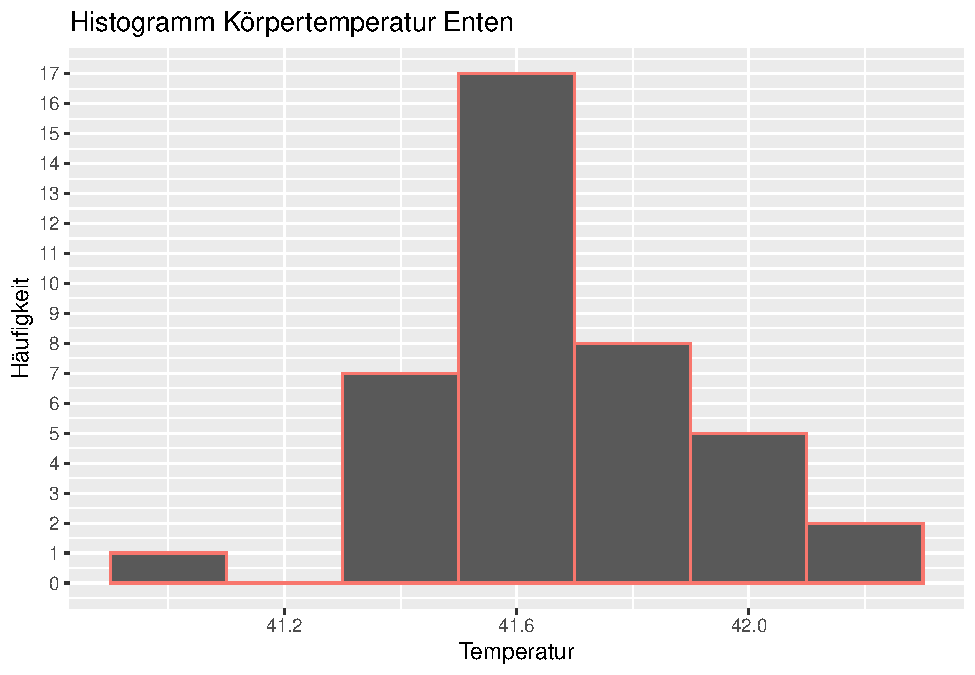
\includegraphics{aps_statistik1_files/figure-latex/enten_histogramm-1.pdf}

Aufgrund dieser Darstellung kann die Veterinärin nun sehen, wie häufig welche Körpertemperaturen sind. Dies wird die \textbf{Verteilung} des Merkmals genannt. Sie bemerkt zum Beispiel, dass Beobachtungen der Körpertemperatur rund um 41.6°C am häufigsten sind und tiefere und höhere Temperaturen seltener vorkommen. Auf einen Blick sieht sie auch, dass die Temperatur aller Enten zwischen 41°C und 42.2°C war.

Die Verteilung eines Merkmals zu kennen ist hilfreich, jedoch in vielen Situationen (z. B. in der Kommunikation) noch zu komplex. Einfacher ist es die Komplexität einer Verteilung auf zwei Faktoren herunterzubrechen: Die Zentralität und die Variabilität eines Merkmals.

\subsection{Zentralität}\label{zentralitaet}

Mit der Zentralität ist ein Wert gemeint, welcher die zentrale Tendenz des Merkmals abbildet. Um die Zentralität zu messen, gibt es drei Möglichkeiten:

\begin{itemize}
\tightlist
\item
  \phantomsection\label{customdef-modus}{Der \textbf{Modus} ist der am häufigsten vorkommende Wert.} Im Beispiel ist das der Wert 41.52, welcher 3 mal und damit am häufigsten vorkommt. In Jamovi wird der Modus mit \texttt{Modalwert} bezeichnet.
\item
  \phantomsection\label{customdef-median}{Wenn die Werte des Merkmals aufsteigend sortiert werden und der Wert betrachtet wird, welcher die Beobachtungen in eine tiefere und eine höhere Hälfte teilt, dann wird dieser Wert als \textbf{Median} (abgekürzt \emph{Mdn}, Symbol \(\tilde{x}\)) bezeichnet.} Bei einer geraden Anzahl Beobachtungen, wird in der Regel der Durchschnittswert der beiden mittigsten Beobachtungen verwendet. Im Beispiel haben wir 40 Beobachtungen. Der Median entspricht also dem Durchschnittswert zwischen dem 20. und dem 21. der aufsteigend sortierten Werte 41.07, 41.32, 41.35, 41.43, 41.46, 41.46, 41.48, 41.5, 41.51, 41.52, 41.52, 41.52, 41.53, 41.53, 41.54, 41.58, 41.58, 41.6, 41.62, 41.65, 41.66, 41.67, 41.67, 41.69, 41.7, 41.72, 41.8, 41.81, 41.81, 41.82, 41.82, 41.88, 41.89, 41.92, 41.92, 41.96, 42.01, 42.06, 42.14 und 42.18, also 41.655. In Jamovi wird der Median mit \texttt{Median} bezeichnet.
\item
  \phantomsection\label{customdef-arithmetisches-mittel}{Das \textbf{arithmetische Mittel} (abgekürzt \emph{M}, Symbol \(\bar{x}\)) bezeichnet, was gemeinhin mit Durchschnitt gemeint ist.} Wenn wir die erste von insgesamt \(n\) Beobachtung mit \(x_1\) und die letzte Beobachtung mit \(x_n\) bezeichnen, so ist das arithmetische Mittel
  \begin{equation}
  \bar{x} = \frac{1}{n}\sum^n_{i=1} x_i
  \label{eq:mean}
  \end{equation}
  Im Beispiel ist das arithmetische Mittel der Körpertemperaturen 41.6725. In Jamovi wird das arithmetische Mittel als \texttt{Mittelwert} bezeichnet.
\end{itemize}

\begin{caution}

\begin{remark}
\emph{Erklärung der Formel}: Hier wird zum ersten Mal eine Formel verwendet. \(\sum\) steht für die Summe von allen Beobachtungen \(x_i\), wenn der Index \(i\) in \(1\)-Schritten von der Zahl unter dem Summenzeichen \(i=1\) bis zu der Zahl oben am Summenzeichen \(i=n\) läuft. In unserem Beispiel ist \(n=40\), also ist \(i = 1, 2, 3, 4, \ldots, 39, 40\). Der Teil \(\sum^n_{i=1} x_i\) bedeutet also nichts anderes als \(x_1 + x_2 + \ldots + x_{39} + x_{40}\), also die Summe aller Beobachtungen. \(\frac{1}{n}\) bedeutet, dass wir diese Summe jetzt noch durch die Anzahl Beobachtungen teilen.

\emph{Welchen Einfluss haben die verschiedenen Einflussgrössen}: Dies wird in Übung \ref{exr:theorie-mdn-mean} erklärt.
\end{remark}

\end{caution}

Jedes dieser Masse für die Zentralität hat Vor- und Nachteile und sie werden dementsprechend in unterschiedlichen Situationen eingesetzt, siehe Übungen.

\subsection{Variabilität}\label{variabilitaet}

\begin{itemize}
\tightlist
\item
  \phantomsection\label{customdef-spannweite}{Die \textbf{Spannweite} (abgekürzt \(R\) aus dem englisch \emph{range}) ist der höchste beobachtete Wert minus der kleinste beobachtete Wert}. Im Beispiel ist der höchste beobachtet Wert \(42.18° C\) und der kleinste Beobachtete Wert \(41.07° C\). Also ist die Spannweite \(42.18 - 41.07 = 1.11° C\). Die Spannweite wird in Jamovi mit \texttt{Wertebereich} bezeichnet.
\item
  \phantomsection\label{customdef-perzentil}{Wenn die Werte des Merkmals aufsteigend sortiert werden und der Wert betrachtet wird, welcher die Beobachtungen in eine \(P\%\) tiefere und \((100\% - P\%)\) höhere Hälfte teilt, dann wird dieser Wert als \textbf{Perzentil} bezeichnet.} Das \(5\%\)-Perzentil zum Beispiel teilt die beobachteten Werte in \(5\%\) kleinere und \(95\%\) grössere Werte. Im Beispiel haben wir 40 Beobachtungen. \(5\%\) davon sind demnach \(2\) Beobachtungen die tiefer sind als das \(5\%\) Perzentil und \(95\%\) also \(38\) Beobachtungen die höher sind als das \(5\%\) Perzentil. Das \(5\%\) Perzentil liegt also zwischen \(41.32° C\) und \(41.35° C\). In diesem Fall wird ein Mittelwert der beiden nächsten Werte verwendet, hier \((41.32 + 41.35)/2=41.34° C\). Das \(P\%\)-Perzentil kann in Jamovi bei \texttt{Perzentil} gefolgt von der Zahl \texttt{P} ermittelt werden. Ein Perzentil alleine gibt jedoch noch keinen Hinweis auf die Streuung der Werte. Werden aber zwei Perzentile zusammen betrachtet, z. B. das \(5\%\) und das \(95\%\) Perzentil, dann geben diese Werte und der Abstand dazwischen einen Hinweis auf die Streuung der Beobachtungen. Im Beispiel ist das \(5\%\) Perzentil bei \(41.34° C\) und das \(95\%\)-Perzentil bei \(42.1° C\). Hier befinden sich also \(90\%\) aller Beobachtungen zwischen diesen Werten. Mehrere Perzentile können in Jamovi gleichzeitig angezeigt werden indem die Perzentil-Werte mit Komma getrennt werden, für die Perzentile hier im Beispiel \texttt{0.05,\ 0.95}. \phantomsection\label{customdef-quartile}{Weitere beliebte Werte sind das \(25\%\) und das \(75\%\)-Perzentil (auch \textbf{Quartile} genannt, da sie die beobachteten Werte vierteln), im Beispiel bei \(41.52° C\) und \(41.82° C\) respektive.} \phantomsection\label{customdef-iqr}{Die Differenz dieser Perzentile wird als \textbf{Interquartilabstand} (abkürzung IQR von interquartile range) bezeichnet und ist im Beispiel \(0.3° C\).}. Der Interquartilabstand wird in Jamovi mit \texttt{IQR} bezeichnet.
\item
  \phantomsection\label{customdef-std}{Die \textbf{Standardabweichung} (abgekürzt \emph{SD}, Symbol \(s\)) ist die durchschnittliche Abweichung jeder Beobachtung vom arithmetischen Mittel.} Wenn wir die erste von insgesamt \(n\) Beobachtung mit \(x_1\) und die letzte Beobachtung mit \(x_n\) bezeichnen, so ist die Standardabweichung
  \begin{equation}
  s = \sqrt{\frac{1}{n-1}\sum^n_{i=1} (x_i-\bar{x})^2}
  \label{eq:sd}
  \end{equation}
  Im Beispiel ist die Standardabweichung der Körpertemperaturen \(0.233° C\). In Jamovi wird die Standardabweichung mit \texttt{Std.-abweichung} bezeichnet.
\end{itemize}

\begin{caution}

\begin{remark}
\emph{Erklärung der Formel}: \((x_i-\bar{x})\) bezeichnet den Abstand von jeder Beobachtung zum arithmetischen Mittel. Dieser Abstand kann positiv (wenn \(x_i\) grösser ist als \(\bar{x}\)) oder negativ (wenn \(x_i\) kleiner ist als \(\bar{x}\)) ausfallen. Damit diese positiven und negativen Abstände sich in der Summe nicht ausgleichen und eine Standardabweichung von 0 entsteht, werden diese Abstände quadriert \((x_i-\bar{x})^2\) bevor sie summiert werden. Anschliessend wird diese Summe durch \(n-1\) geteilt, um den durchschnittlichen Abstand pro Beobachtung zu ermitteln. Intuitiv würde man hier durch \(n\) teilen. Statistiker:innen haben jedoch herausgefunden, dass es einige Vorteile hat, wenn durch \(n-1\) statt \(n\) geteilt wird. Das Quadrat wird nach der Aufsummierung wieder aufgehoben indem die Quadratwurzel gezogen wird.
\end{remark}

\end{caution}

\section{Übungen}\label{intervallskaliertes-merkmal-uebungen}

\begin{exercise}
\protect\hypertarget{exr:enten-hist-mean-sd}{}\label{exr:enten-hist-mean-sd}\leavevmode

Mit den Daten \texttt{02-exm-ducktemp.sav} aus Beispiel \ref{exm:ducktemp}:

\begin{enumerate}
\def\labelenumi{(\alph{enumi})}
\tightlist
\item
  Erstellen Sie selbst ein Histogramm mit Jamovi und begründen Sie, weshalb es nicht gleich aussieht wie das Histogramm oben.
\item
  Berechnen Sie zusätzlich Modus, Median, arithmetisches Mittel, IQR, 25\%- und 75\%-Perzentil, sowie 2.5\%- und 97.5\%-Perzentil, sowie die Spannweite und die Standardabweichung der Körpertemperaturen der Enten mit Jamovi.
\end{enumerate}

\end{exercise}

\begin{solution}
\leavevmode

\begin{figure}
  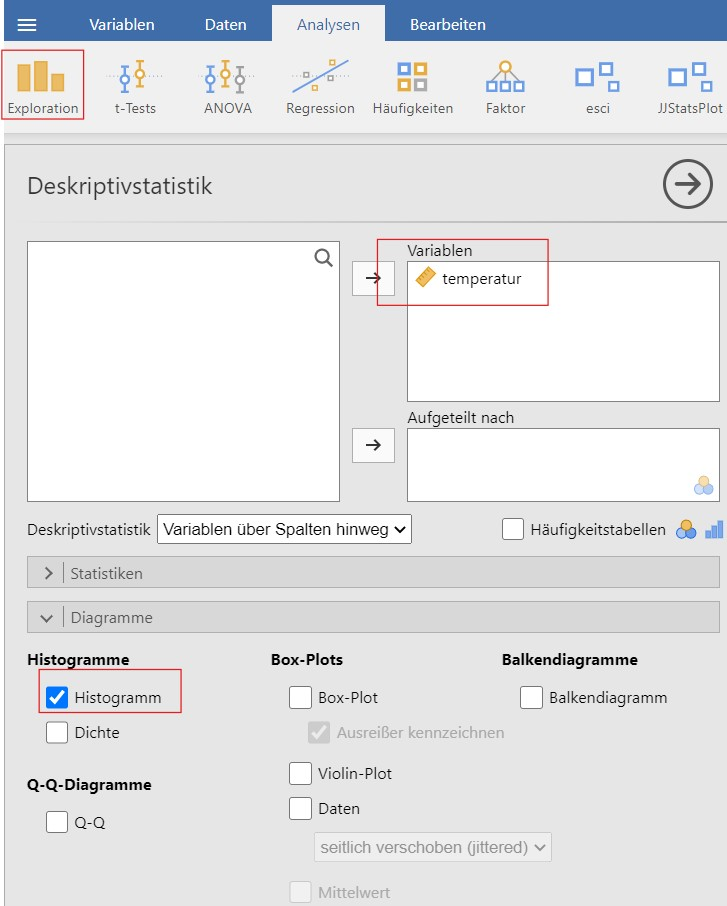
\includegraphics[width=0.5\linewidth]{figures/Enten_n40_instr_histogramm} 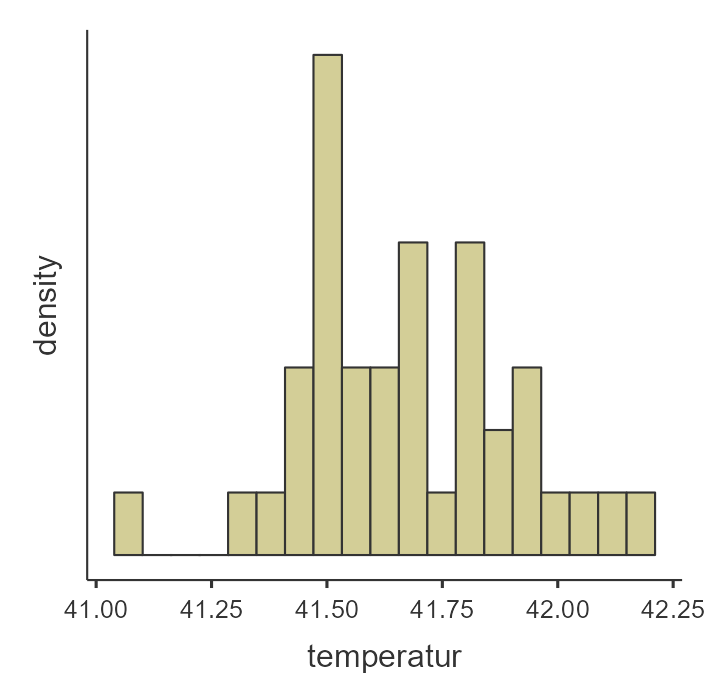
\includegraphics[width=0.5\linewidth]{figures/Enten_n40} \caption{Links: Jamovi-Anleitung zur Erstellung des Histogramms; rechts: Histogramm der Temperatur.}\label{fig:enten-hist-mean-sd1}
  \end{figure}

\begin{enumerate}
\def\labelenumi{(\alph{enumi})}
\tightlist
\item
  Das Histogramm, siehe Abbildung \ref{fig:enten-hist-mean-sd1} sieht nicht gleich aus, da Jamovi die Temperaturabschnitte kürzer gewählt hat nämlich bei 0.125°C statt 0.2°C wie oben im Text. In Jamovi gibt es aktuell keine Möglichkeit die Abschnittsweite anzupassen. Ein Histogramm sieht immer anders aus je nach ausgewählter Abschnittsweite.
\end{enumerate}

\begin{figure}
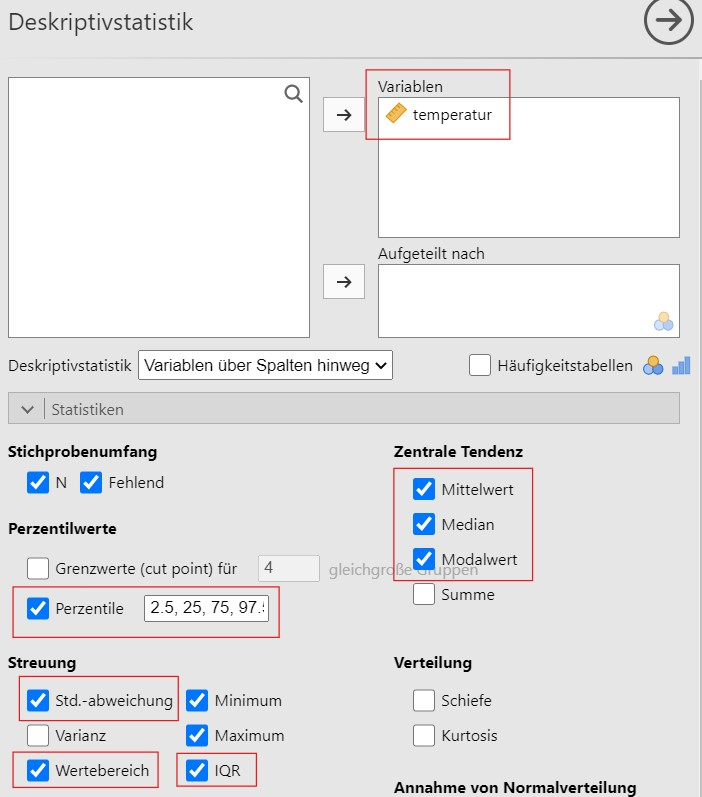
\includegraphics[width=0.5\linewidth]{figures/02-exr-enten-hist-mean-sd-input} 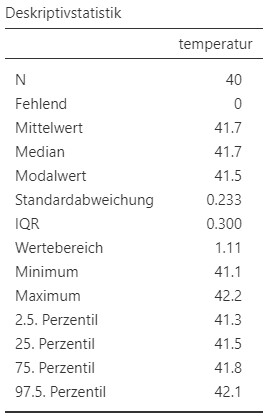
\includegraphics[width=0.5\linewidth]{figures/02-exr-enten-hist-mean-sd-output} \caption{Links: Jamovi-Anleitung zur Berechnung der gewünschten Parameter; rechts: Parameterwerte.}\label{fig:enten-hist-mean-sd2}
\end{figure}

\begin{enumerate}
\def\labelenumi{(\alph{enumi})}
\setcounter{enumi}{1}
\tightlist
\item
  Eine Anleitung zur Berechnung in Jamovi sowie die berechneten Werte können in Abbildung \ref{fig:enten-hist-mean-sd2} abgelesen werden.
\end{enumerate}

\end{solution}

\begin{exercise}
\protect\hypertarget{exr:temptag_pvai8hwv}{}\label{exr:temptag_pvai8hwv}\leavevmode

TODO: Exercise body

\end{exercise}

\begin{solution}
TODO: solution body
\end{solution}

\begin{exercise}
\protect\hypertarget{exr:theorie-mdn-mean}{}\label{exr:theorie-mdn-mean}\leavevmode

In einem psychologischen Test machen \(5\) Probandinnen die Werte \(18, 21, 20, 19, 22\). Um mit einer Zahl zu sagen, wo die Testresultate liegen, wird ein zentraler Wert berechnet.

\begin{enumerate}
\def\labelenumi{(\alph{enumi})}
\tightlist
\item
  Wie gross ist das arithmetische Mittel und der Median dieser Werte?
\item
  Nehme an, der Testleiter hat den Wert der ersten Probandin falsch in seine Tabelle übertragen - statt \(18\) hat er \(81\) geschrieben. Wie gross ist das arithmetische Mittel und der Median dieser Werte in diesem Fall?
\item
  Was sagt dies über den Median und das arithmetische Mittel aus?
\end{enumerate}

\end{exercise}

\begin{solution}

Die Aufgabe kann im Kopf gelöst werden, oder mithilfe eines Taschenrechners, oder indem die Zahlen manuell bei Jamovi eingegeben werden.

\begin{enumerate}
\def\labelenumi{(\alph{enumi})}
\tightlist
\item
  Wir haben hier \(n=5\) Beobachtungen, nämlich \(x_1 = 18, x_2 = 21, x_3 = 20, x_4 = 19, x_5=22\). Wird dies in die Formel \eqref{eq:mean} eingesetzt, so gibt dies das arithmetische Mittel
  \[\bar{x} = \frac{1}{n}\sum^n_{i=1} x_i = \frac{1}{n}(x_1 + x_2 + x_3 + x_4 + x_5) =  \frac{1}{5}(18+ 21+ 20+ 19+ 22) = 20.\]
  Um den Median zu berechnen, werden die Werte zuerst aufsteigend sortiert \(18, 19, 20, 21, 22\). Der Wert, welcher die Werte in eine grössere und eine kleinere Hälfte teilt, ist hier \(20\), was dem Median entspricht.
\item
  Die Beobachtungen sind jetzt \(x_1 = 81, x_2 = 21, x_3 = 20, x_4 = 19, x_5=22\). Analog wie in (a) kann demnach das arithmetische Mittel als \(\bar{x} = 32.6\) bestimmt werden. Die aufsteigend sortierten Beobachtungen sind nun \(19, 20, 21, 22, 81\). Der Median ist also \(21\).
\item
  Durch die fälschliche Übertragung eines Wertes, ist das arithmetische Mittel sehr stark und der Median fast gar nicht beeinflusst worden. Wenn die Daten wenige fehlerhafte Beobachtungen enthalten, ist der Median das bessere Mass für den zentralen Wert als das arithmetische Mittel. Wenn die Daten keine Fehler enthalten, ist das arithmetische Mittel gleich gut geeignet wie der Median.
\end{enumerate}

\end{solution}

\begin{exercise}
\protect\hypertarget{exr:temptag_poiane}{}\label{exr:temptag_poiane}\leavevmode

TODO: Exercise body

\end{exercise}

\begin{solution}
TODO: solution body
\end{solution}

\begin{exercise}
\protect\hypertarget{exr:diverse-distrib}{}\label{exr:diverse-distrib}\leavevmode

Für eine Studie werden Studierende gebeten eine Aufgabe zu lösen, bei welcher Sie eine gewisse Anzahl \texttt{Punkte} erzielen. Über jede Proband:in sind ausserdem folgende Eigenschaften bekannt:

\begin{itemize}
\tightlist
\item
  \texttt{IQ}: Intelligenzquotient
\item
  \texttt{Aufgeschlossenheit}: Likert von 1-7
\item
  \texttt{Wartezeit\_min}: Wartezeit vor beginn des Experiments in Minuten
\item
  \texttt{Wartezeit\_std}: Wartezeit vor beginn des Experiments in Stunden
\item
  \texttt{Geburtzeit\_std\_ab\_mitternacht}: Geburtszeit in Stunden ab Mitternacht. Wenn jemand um 13h30 auf die Welt kam, ist dieser Wert 13.5.
\item
  \texttt{Geburtzeit\_std\_ab\_mittag}: Geburtszeit in Stunden ab Mittag. Wenn jemand um 13h30 auf die Welt kam, ist dieser Wert 1.5.
\end{itemize}

Die Daten sind in Jamovi unter \texttt{02-exr-diverse-distrib.sav} verfügbar.

Analysieren Sie alle erhobenen Merkmale indem Sie ein Histogramm erstellen und die zentralen Tendenzen sowie die Variabilität analysieren.

\begin{enumerate}
\def\labelenumi{\alph{enumi}.}
\tightlist
\item
  Wie viele Personen nahmen an der Studie teil?
\item
  Vergleichen Sie Ihre Ergebnisse für die Merkmale IQ und Aufgeschlossenheit. Was für Zusammenhänge fallen auf?
\item
  Vergleichen Sie Ihre Ergebnisse für die Wartezeiten Merkmale. Was für Zusammenhänge fallen auf?
\item
  Vergleichen Sie Ihre Ergebnisse für die Merkmale Punkte und Wartezeiten. Was für Zusammenhänge fallen auf?
\item
  Geburtszeit. TODO.
\end{enumerate}

\end{exercise}

\begin{solution}
\leavevmode

\begin{figure}
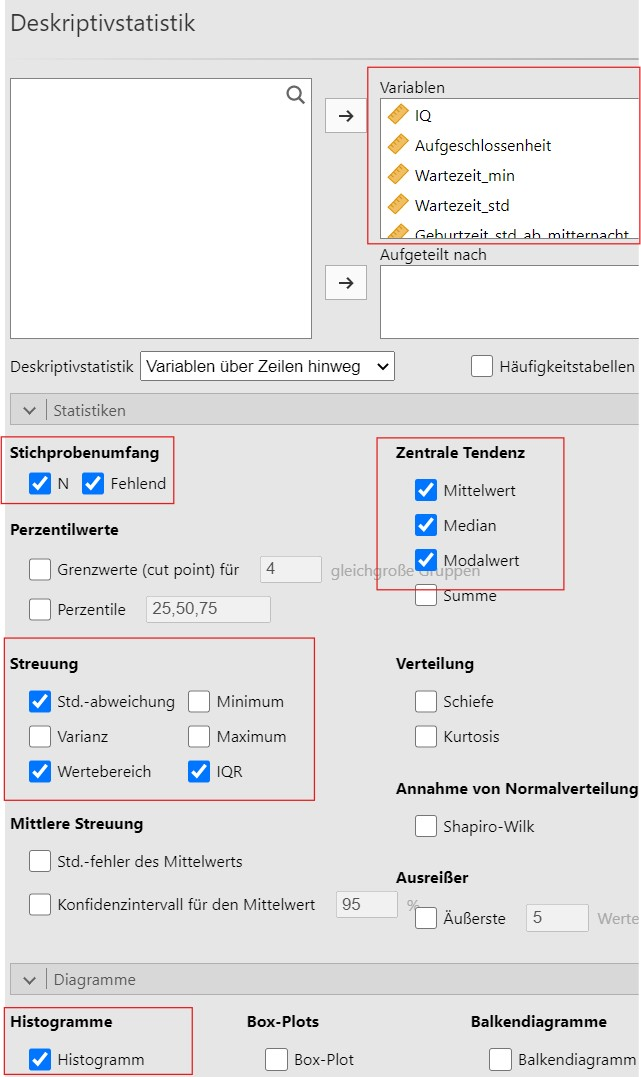
\includegraphics[width=1\linewidth]{figures/02-exr-diverse-distrib-input} \caption{Jamovi Eingabe.}\label{fig:sol-diverse-distrib1}
\end{figure}

\begin{figure}
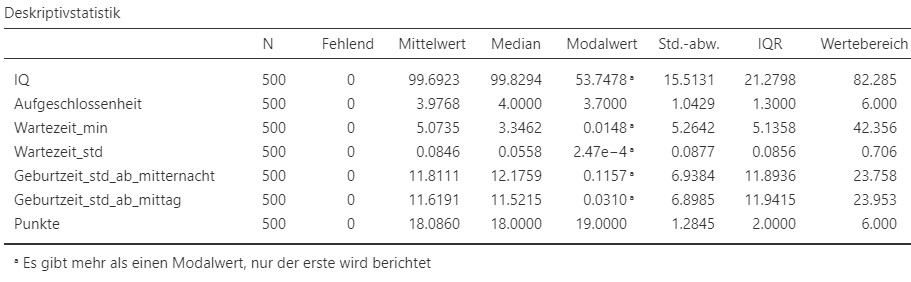
\includegraphics[width=1\linewidth]{figures/02-exr-diverse-distrib-output} \caption{Deskriptive Statistiken.}\label{fig:sol-diverse-distrib2}
\end{figure}

\begin{figure}
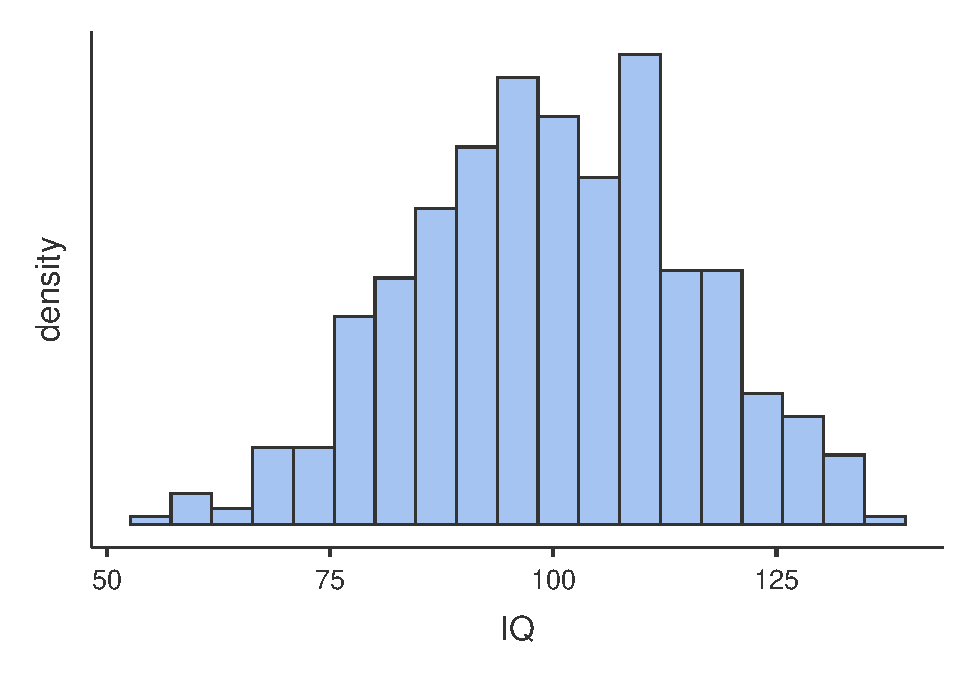
\includegraphics[width=0.33\linewidth]{aps_statistik1_files/figure-latex/sol-diverse-distrib3-1} 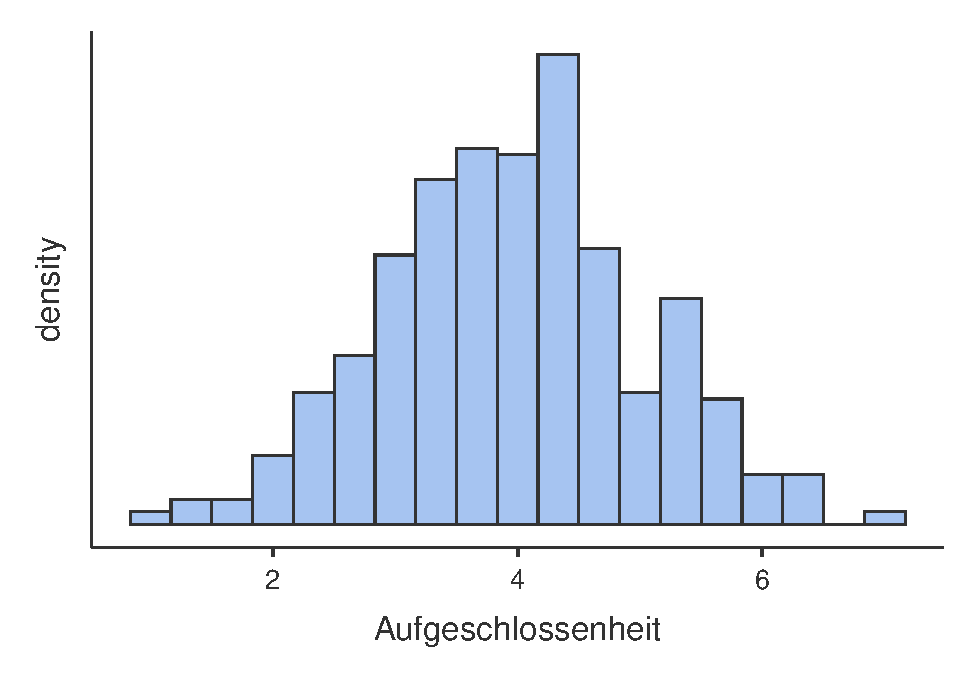
\includegraphics[width=0.33\linewidth]{aps_statistik1_files/figure-latex/sol-diverse-distrib3-2} 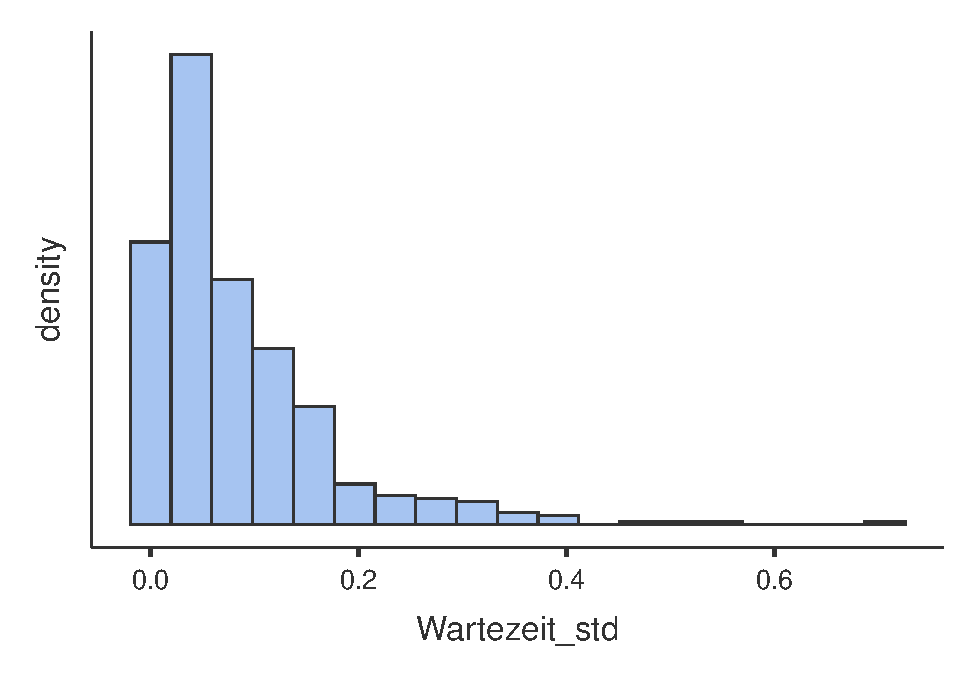
\includegraphics[width=0.33\linewidth]{aps_statistik1_files/figure-latex/sol-diverse-distrib3-3} 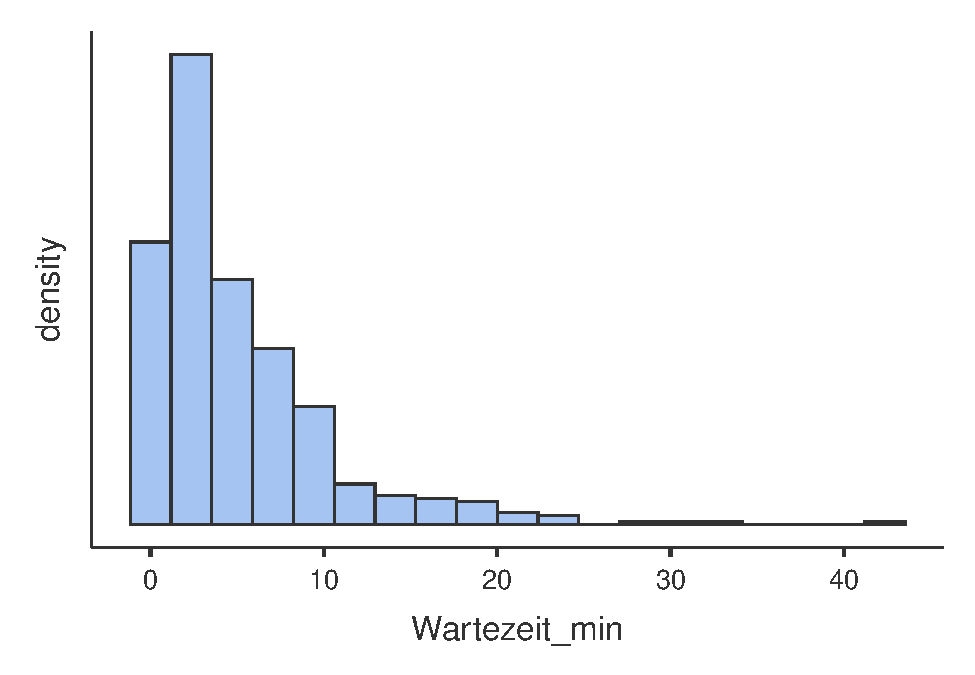
\includegraphics[width=0.33\linewidth]{aps_statistik1_files/figure-latex/sol-diverse-distrib3-4} 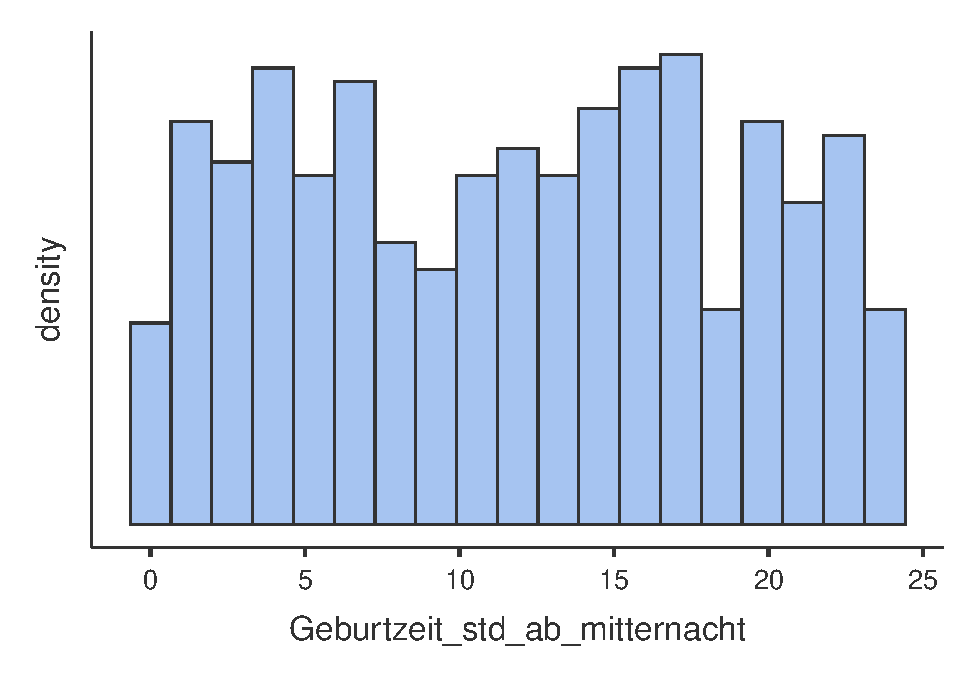
\includegraphics[width=0.33\linewidth]{aps_statistik1_files/figure-latex/sol-diverse-distrib3-5} 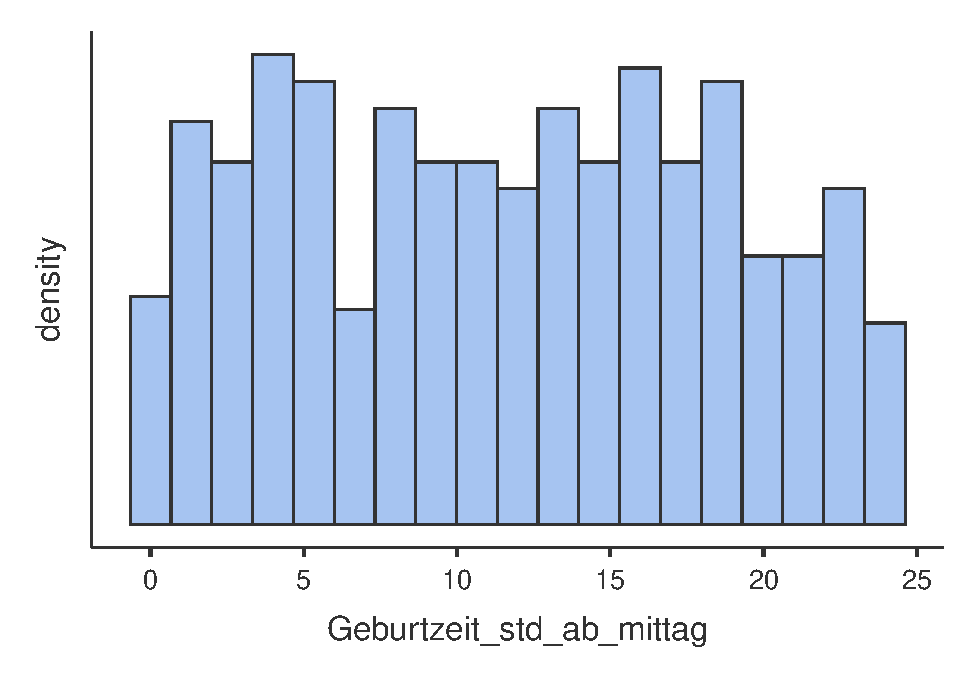
\includegraphics[width=0.33\linewidth]{aps_statistik1_files/figure-latex/sol-diverse-distrib3-6} 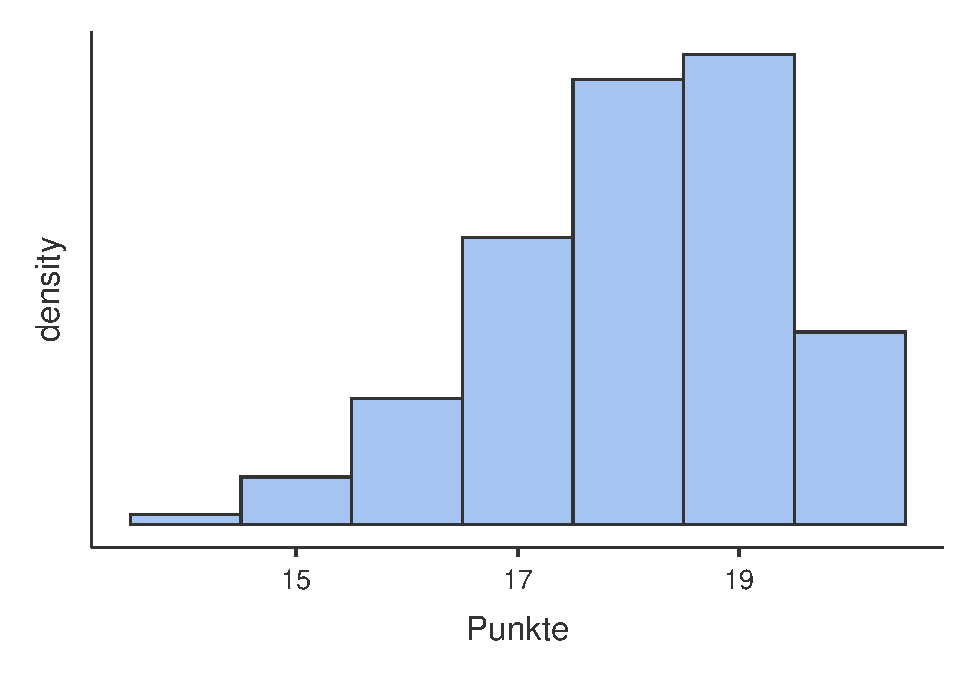
\includegraphics[width=0.33\linewidth]{aps_statistik1_files/figure-latex/sol-diverse-distrib3-7} \caption{Histogramme.}\label{fig:sol-diverse-distrib3}
\end{figure}

Die Merkmale werden mit den Befehlen in Abbildung \ref{fig:sol-diverse-distrib1} analysiert.

\begin{enumerate}
\def\labelenumi{\alph{enumi}.}
\tightlist
\item
  Es gibt gemäss \ref{fig:sol-diverse-distrib2} genau \(500\) Studienteilnehmende (siehe \(N\)).
\item
  Die Histogramme für den IQ und die Aufgeschlossenheit weisen eine ähliche Form auf. Viele Beobachtungen sind um eine Mitte zentriert. Je weiter weg von der Mitte, desto seltener sind die Beobachtungen. Das Histogram des IQ zeigt, dass die Verteilung rund um 100 zentriert ist und ca von 60 bis 140 reicht. Je weiter entfernt von 100, desto weniger Beobachtungen wurden gemacht. Das Histogram der Aufgeschlossenheit stellt dar, dass diese rund um 4 zentriert ist mit Werten von 1 bis 7. Je weiter die Werte von 4 entfernt sind, desto weniger häufig sind die Beobachtungen. Der vom Histogram abgeleitete vorher genannte zentrale Wert entspricht ungefähr dem Mittelwert und dem Median für beide Merkmale. Für die Aufgeschlossenheit hat der Modalwert ebenfalls einen ähnlichen Wert. Der Modus für den IQ ist nicht belastbar, da die Fussnote besagt, dass mehrere Werte als Modus in Frage kommen. Eine genauere Durchsicht der IQ-Werte lässt folgern, dass aufgrund der vielen Nachkommastellen jeder IQ-Wert nur genau einmal vorkommt. Der angebene Modalwert des IQs entspricht also einfach einer zufälligen Beobachtung. Die Kennwerte für die Variabilität lassen ebenfalls auf Unterschiede zwischen den beiden Merkmalen schliessen. Die höheren Werte Standardabweichung, IQR und Wertebereich des IQ im Vergleich zur Aufgeschlossenheit legen nahe, dass die Streuung der Werte für den IQ viel grösser ist. Zum Beispiel ist eine durchschnittliche IQ-Beobachtung 15.5 IQ-Werte weg vom durchschnittlichen IQ und eine durchschnittliche Aufgeschlossenheits-Beobachtung nur 1.3 Aufgeschlossenheits-Werte weg von der duchschnittlichen Aufgeschlossenheit. Dies ist auf dem Histogramm zu erkennen, wenn die Skala der horizontalen Achse betrachtet wird. Für den IQ reicht diese von 50 bis 125 und für die Aufgeschlossenheit von 2 bis 6.
\item
  Die Wartezeiten wurden einmal in Minuten und einmal in Stunden abgespeichtert. Die resultierenden Histogramme sind deshalb genau identisch bis auf die Werte der horizontalen Achse, welche von 0 bis 0.6 Stunden und von 0 bis 40 Minuten reicht. Im Vergleich zu den Histogrammen des IQ und der Aufmerksamkeit kann für die Wartezeit und eine asymetrische Verteilung beobachtet werden. Kurze Wartezeiten werden demnach häufiger beobachtet als längere Wartezeiten. Die meisten Wartezeiten liegen unter 10 Minuten, sehr selten kommt es zu Wartezeiten über 20 Minuten. Die Kennzahlen für die Wartezeit in Stunden können aus den Kennzahlen der Wartezeit in Stunden hergeleitet werden indem die Werte durch \(60\) geteilt werden. Es reicht deshalb die Kennzahlen für die Wartezeit in Minuten zu betrachten. Die durchscnittliche Wartezeit liegt bei \(M=5.07, Mdn = 3.97\) Minuten. Der Modalwert ist wiederum nicht interpretierbar aus demselben Grund wie oben. Der Median bedeutet, dass \(50\%\) der Wartezeiten kleiner und \(50\%\) der Wartezeiten grösser waren als \(3.97\) Minuten. Das arithmetische Mittel ist höher als der Median. Die einigen wenigen Beobachtungen mit sehr langen Wartezeiten haben also das arithmetische Mittel im Vergleich zum Median stärker beeinflusst.
\item
  TODO.
\item
  TODO: Zentraler Wert hier nicht identifiziertbar, streuung auch nicht.
\end{enumerate}

\end{solution}

\chapter{Stichprobenziehung}\label{stichprobenziehung}

\begin{example}[Angst]
\protect\hypertarget{exm:angst}{}\label{exm:angst}Forschende haben ein Messinstrument State-Trait Anxiety Inentory \emph{STAI}, welches Angst misst \citep{spielberger1983manual}. Sie unterscheiden dabei zwischen Zustandesangst und dem Persönlichkeitszug Ängslichkeit. Hier interessiert uns nur die Zustandesangst, welche fortan Angst genannt wird und misst wie grosse Angst man aktuell empfindet. Die so gemessene Angst enstpricht einem Wert zwischen \(20\) und \(80\). A priori haben die Forschenden keine Ahnung, wie viel Angst eine Person im Durchschnitt hat und ob die ganze Skala der Werte genutzt wird. Die Forschenden machen deshalb eine kleine Befragung mit \(n =30\) zufällig ausgewählten Studierenden. Die Forschenden finden die zusammenfassenden Werte \(M=43.34, s = 9.72, n = 30\) für die Angst in ihren Beobachtungen.
\end{example}

\phantomsection\label{customdef-stichprobe}{Zufällig ausgewählte Beobachtungen eines Merkmals werden als \textbf{Stichprobe} bezeichnet.} \phantomsection\label{customdef-stichprobenziehung}{Nach der Auswahl der Stichprobe ist die \textbf{Stichprobenziehung}.} Ist mit diesen Beobachtungen die Aussage beschränkt auf die Stichprobe oder kann damit auch eine Aussage zur Angst für alle Personen getroffen werden? \phantomsection\label{customdef-population}{Alle Personen, oder generell alle möglichen Beobachtungen eines Merkmals, werden als \textbf{Population}} \phantomsection\label{customdef-grundgesamtheit}{oder \textbf{Grundgesamtheit} bezeichnet}. \phantomsection\label{customdef-zufallsstichprobe}{Eine Stichprobe ist für viele Analyseverfahren repräsentativ für eine Population, wenn sie zufällig aus dieser Population gezogen. Ist dies gegeben, wird die Stichprobe auch als \textbf{Zufallsstichprobe} bezeichnet.}

\begin{remark}
Viele Studien basieren auf Testresultaten von Studierenden, weil diese nahe am Forschungsbetrieb sind und damit über Studien informiert sind oder für wenig Geld oder Bildungsanerkennung an Studien teilnehmen. Einige dieser Studien generalisieren ihre Forschungsresultate nachher auf alle Personen. Dies ist in der Regel falsch, da Studierende nicht repräsentativ für die Gesamtbevölkerung sind (Altersstruktur, Geschlechtsverteilung, Vermögen, usw.). Die Frage, wie eine repräsentative Stichprobe würde den Rahmen dieses Buches sprengen.
\end{remark}

\section{Was ist das Problem der Stichprobenziehung?}\label{stichprobenziehung-problem}

Es wird angenommen, dass sich alle Personen der Population in einem Zimmer befinden. In Abbildung \ref{fig:srs-intervall-nocol} ist dieses Zimmer aus der Vogelperspektive dargestellt, wobei jeder Punkt im schwarzen Kasten einer Person der Population. Die Personen im Zimmer, respektive die Beobachtungen in der Population sind normalerweise nicht sichtbar. Aus diesem Zimmer wurden also 30 Personen geholt und befragt also sichtbar gemacht, was der Zufallsstichprobe entspricht. Die Zufallsstichprobe ist gekennzeichnet durch die Punkte über dem Zimmer, oberhalb des Pfeils. Die Farben der Punkte sind jetzt bekannt und entsprechen der jeweiligen Zustandesangst der beobachteten Personen.

\begin{figure}
\centering
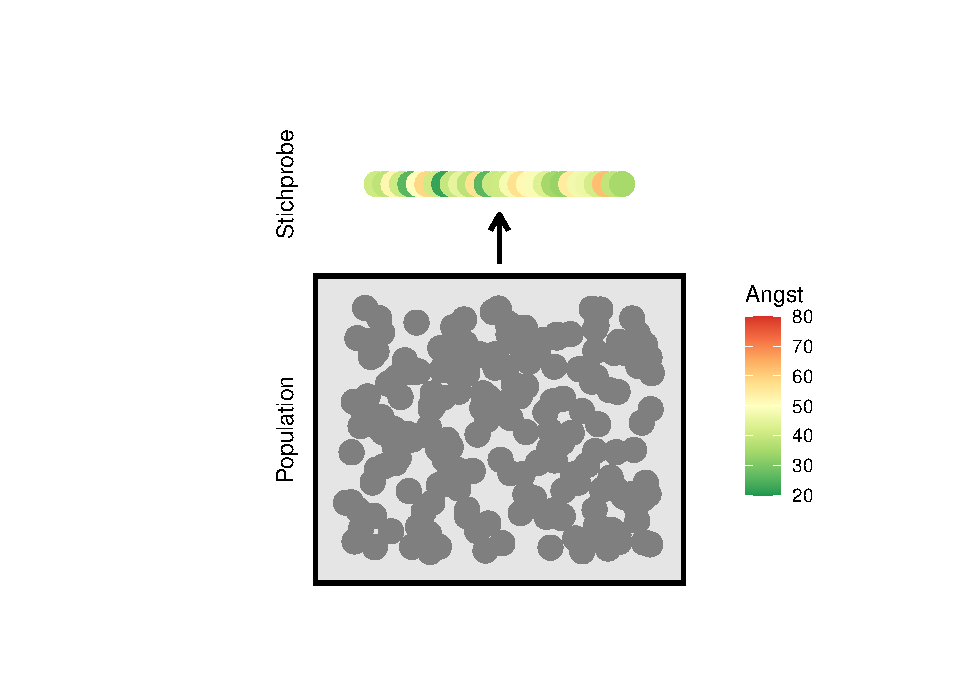
\includegraphics{aps_statistik1_files/figure-latex/srs-intervall-nocol-1.pdf}
\caption{\label{fig:srs-intervall-nocol}Population mit unbekannter Angst.}
\end{figure}

Da die Stichprobe nun eben zufällig gezogen wurde, das heisst zufällig Personen aus dem Zimmer geholt wurden, kann es nun sein, dass die Stichprobe einer Population wie in Abbildung \ref{fig:srs-intervall-high-p} entstammt.

\begin{figure}
\centering
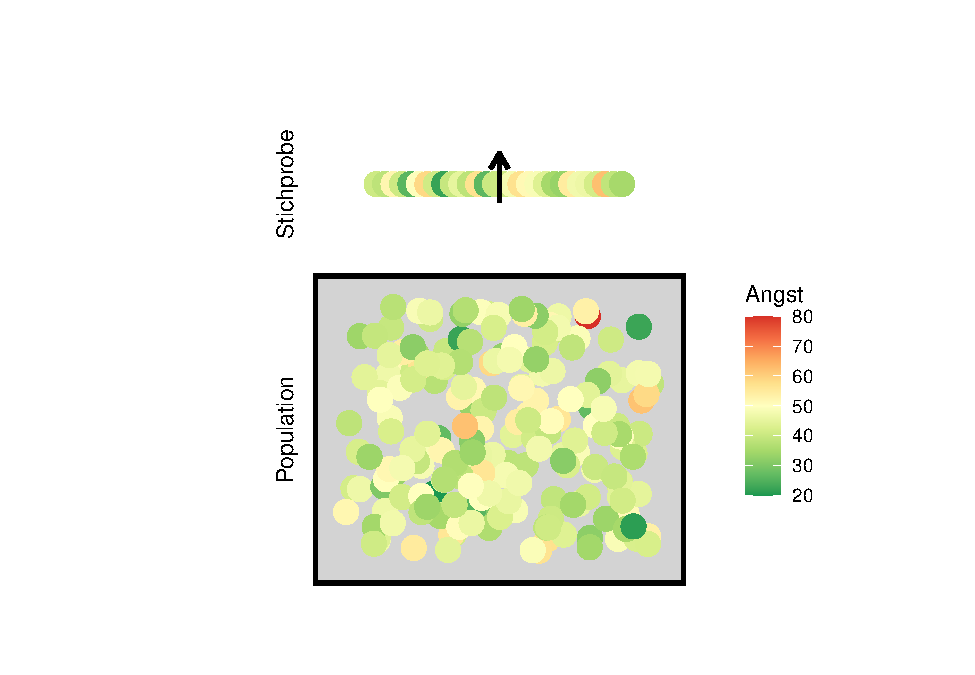
\includegraphics{aps_statistik1_files/figure-latex/srs-intervall-high-p-1.pdf}
\caption{\label{fig:srs-intervall-high-p}Population mit ähnlichen Angst-Werten wie in der Stichprobe.}
\end{figure}

Es könnte aber auch sein, dass die Stichprobe einer Population mit viel höherer Zusatandsangst, wie in Abbildung \ref{fig:srs-intervall-low-p} dargestellt, entstammt. Dies wird zwar weniger häufig vorkommen als der Fall oben, aber ist trotzdem möglich.

\begin{figure}
\centering
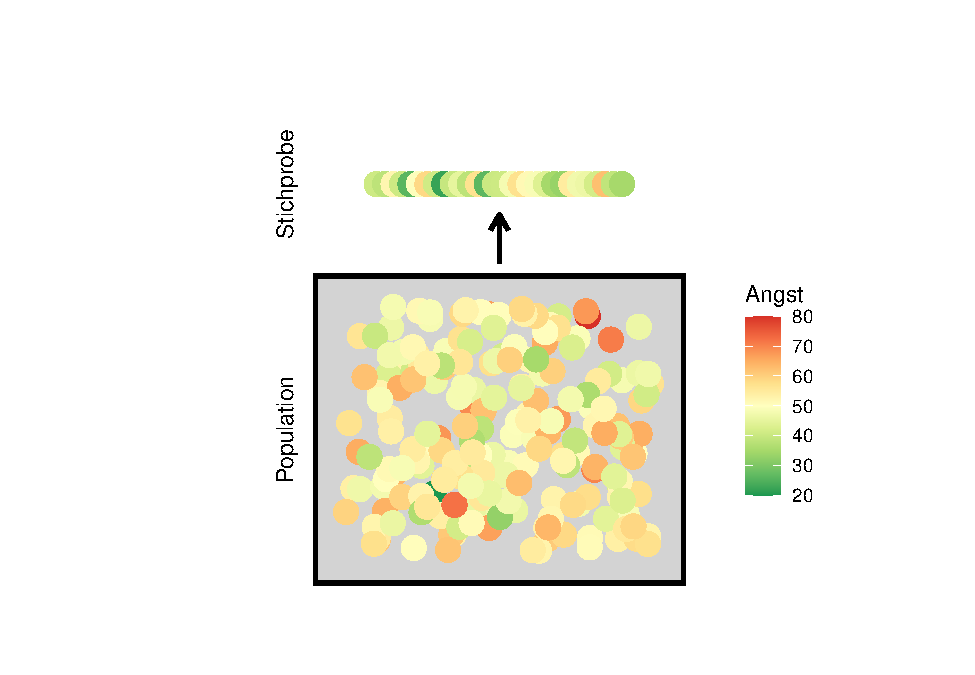
\includegraphics{aps_statistik1_files/figure-latex/srs-intervall-low-p-1.pdf}
\caption{\label{fig:srs-intervall-low-p}Population mit höheren Angst-Werten als in der Stichprobe.}
\end{figure}

Das Problem der zufälligen Stichprobenziehung ist also, dass nie ganz klar ist, wie die darunterliegende Population aussieht. Sind die Werte der Stichprobe tief, weil zufällig gerade Studierende mit tiefer Angst beobachtet wurden, oder haben tatsächlich die meisten Studierenden eine tiefe Angst?

\section{Wie kann man Aussagen über die Grundgesamtheit machen?}\label{stichprobenziehung-loesung}

Die Lösung dieses Problems funktioniert intuitiv wie folgt: Man stellt sich vor, die Stichprobenziehung würde erneut gemacht, und dann nochmal und dann nochmal. So oft, bis man einen guten Eindruck davon hat, wie häufig eine Stichprobe mit eher tiefen Angst-Werten wie bei der Stichprobe im Beispiel vorkommt. Im Szenario, in welchem in der Population tatsächlich tiefe Werte häufig vorkommen, kann dies aussehen wie in Abbildung \ref{fig:srs-intervall-high-p-many}. Stichproben mit eher tiefen Angst-Werten kommen hier häufig vor.

\begin{figure}
\centering
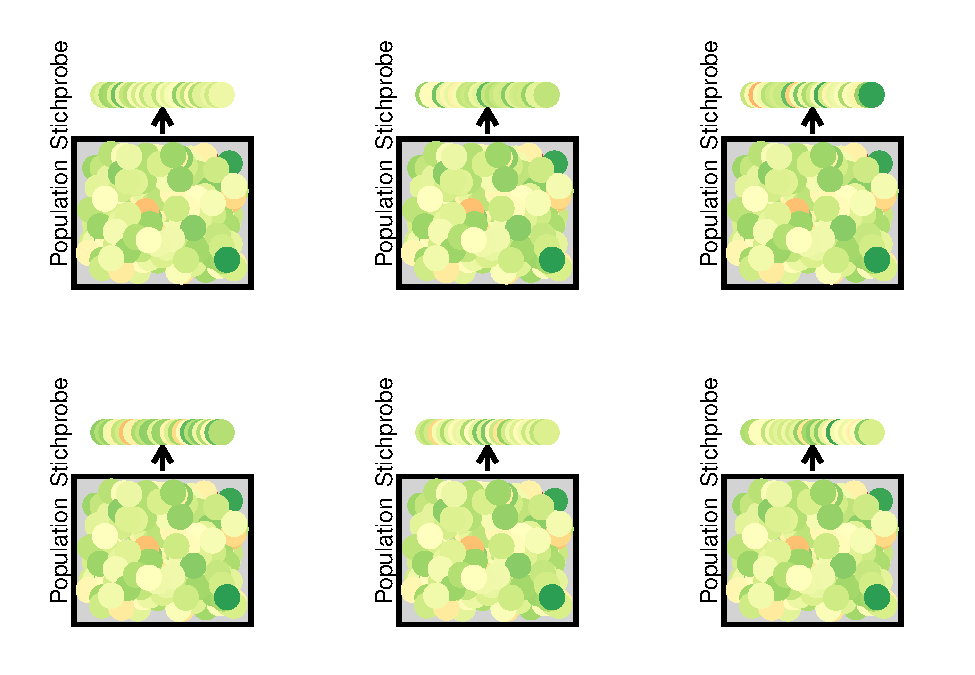
\includegraphics{aps_statistik1_files/figure-latex/srs-intervall-high-p-many-1.pdf}
\caption{\label{fig:srs-intervall-high-p-many}TODO.}
\end{figure}

Im Szenario, in welchem in der Population tatsächlich höhere Werte häufig vorkommen, kann dies aussehen wie in Abbildung \ref{fig:srs-intervall-low-p-many}. Stichproben mit eher tiefen Angst-Werten kommen hier selten oder gar nicht vor.

\begin{figure}
\centering
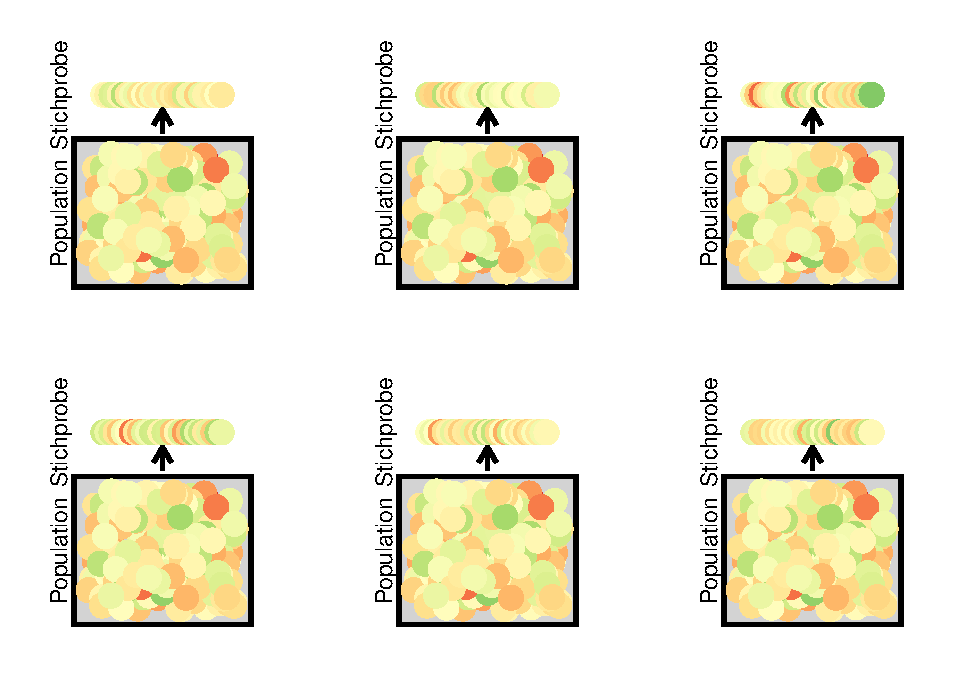
\includegraphics{aps_statistik1_files/figure-latex/srs-intervall-low-p-many-1.pdf}
\caption{\label{fig:srs-intervall-low-p-many}TODO.}
\end{figure}

Es kann also zusammenfassend gesagt werden, dass die gezogene Stichprobe wohl eher aus einer Population mit tiefen Angst-Werten gezogen wurde als aus einer Population mit eher höheren Angst-Werten. Ganz sicher kann man jedoch nie sein, da die Werte in der Population eigentlich unbekannt sind. Eine genaue Quantifizierung dieser Unsicherheit kann mit Hilfe der Statistik erreicht werden und wird in den folgenden Kapiteln dieses Buches erläutert.

\section{Übungen}\label{uxfcbungen}

\begin{exercise}
\protect\hypertarget{exr:tagname_alskfdieu}{}\label{exr:tagname_alskfdieu}\leavevmode

TODO: Exercise body

\end{exercise}

\begin{solution}
TODO: solution body
\end{solution}

\begin{exercise}
\protect\hypertarget{exr:tagname_apwioev}{}\label{exr:tagname_apwioev}\leavevmode

TODO: Exercise body

\end{exercise}

\begin{solution}
TODO: solution body
\end{solution}

\chapter{Durchschnitt und Standardabweichung schätzen}\label{durchschnitt-und-standardabweichung-schuxe4tzen}

Wie die in Abschnitt \ref{stichprobenziehung-loesung} skizzierte Lösung für das Problem der zufälligen Stichprobe konkret umgesetzt wird, hängt von der Problemstellung ab. Im folgenden wird ein Verfahren zur Generalisierung der Schätzung der zentralen Tendenz
basierend auf einer Stichprobe präsentiert.

\section{Wo liegt der Durchschnitt der Grundgesamtheit?}\label{wo-liegt-der-durchschnitt-der-grundgesamtheit}

Ein Parameter über welchen wir gerne eine Aussage treffen würden ist die zentrale Tendenz in der Grundgesamtheit. \phantomsection\label{customdef-erwartungswert}{Diese wird \textbf{Erwartungswert} (Symbol \(\mu\) {[}gr.: mü{]}) genannt.} Wenn das arithmetische Mittel der Stichprobe berechnet wird, ergibt dies auch ein Schätzwert für besagten Erwartungswert. Aufgrund der zufälligen Stichprobenziehung ist jedoch auch klar, dass dieser Schätzwert nie genau dem wahren Erwartungswert entspricht.

In Beispiel \ref{exm:angst} liegt das arithmetische Mittel in der Stichprobe der Studierenden bei \(M=43.2\). Dieser Wert entspricht nun auch der Schätzung des Erwartungswertes, also der geschätzten durchschnittlichen Angst aller Menschen. Die Folgefrage ist also wie genau unsere Schätzung ist. Um dies zu quantifizieren, wiederholen wir die Stichprobenziehung und berechnen das arithmetische Mittel dieser zweiten Stichprobe. Dann wiederholen wir diesen Prozess, zum Beispiel \(1000\) mal.

\begin{figure}
\centering
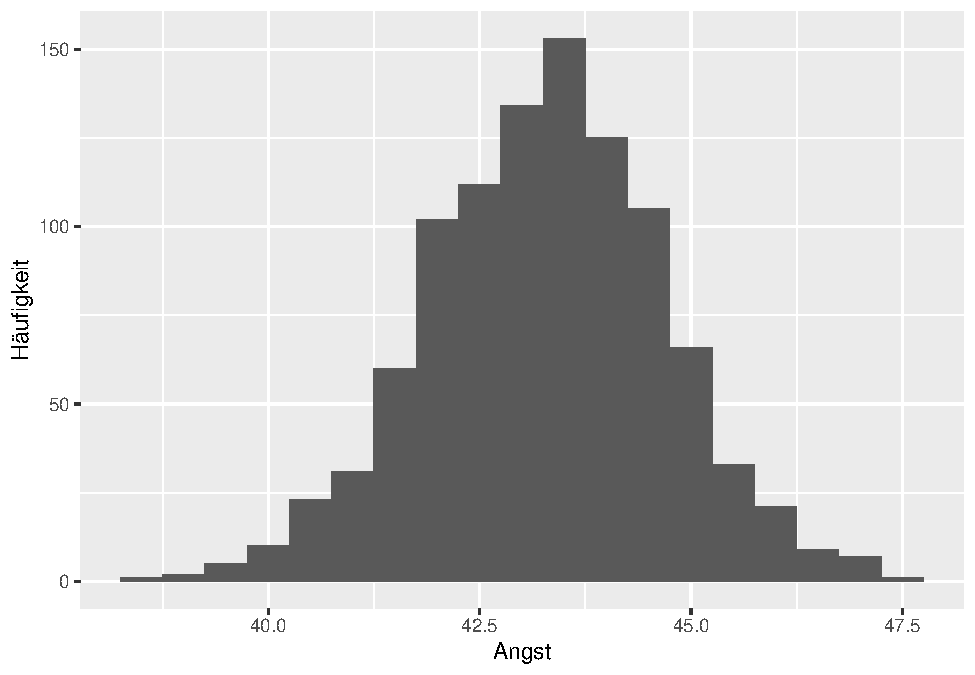
\includegraphics{aps_statistik1_files/figure-latex/exm-angst-hist-means-1.pdf}
\caption{\label{fig:exm-angst-hist-means}Verteilung der arithmetischen Mittel von 1000 zufällig gezogenen Stichproben der Angst.}
\end{figure}

Die Häufigkeitsverteilung der berechneten arithmetischen Mittel in Abbildung \ref{fig:exm-angst-hist-means} lässt nun Aussage über die Häufigkeit und damit über die Wahrscheinlichkeit von gewissen Werten als Erwartungswert zu. Ein Durchschnittswert der Zustandesangst um die 30 ist hier am wahrscheinlichsten und ein Wert tiefer als \(27\) oder höher \(33\) eher selten. Um diese Aussage präziser zu gestalten, werden konventionell die \(95\)\% häufigsten Werte (die höchsten Balken im Histogramm) als wahrscheinlich betrachtet. Die \(5\)\% verbleibenden Werte, verteilt auf das untere und obere Extrem, werden als unwahrscheinlich betrachtet. Das \(2.5\)\% Perzentil trennt die \(2.5\)\% tiefsten arithmetischen Mittel ab und liegt im Beispiel bei \(40.4\). Das \(97.5\)\%-Perzentil trennt die höchsten \(2.5\)\% (oder eben die tiefsten \(97.5\)\%) arthmetischen Mittel ab und liegt bei \(46\). Dies ist in Abbildung \ref{fig:exm-angst-hist-means-emp-ci} ersichtlich.

\begin{figure}
\centering
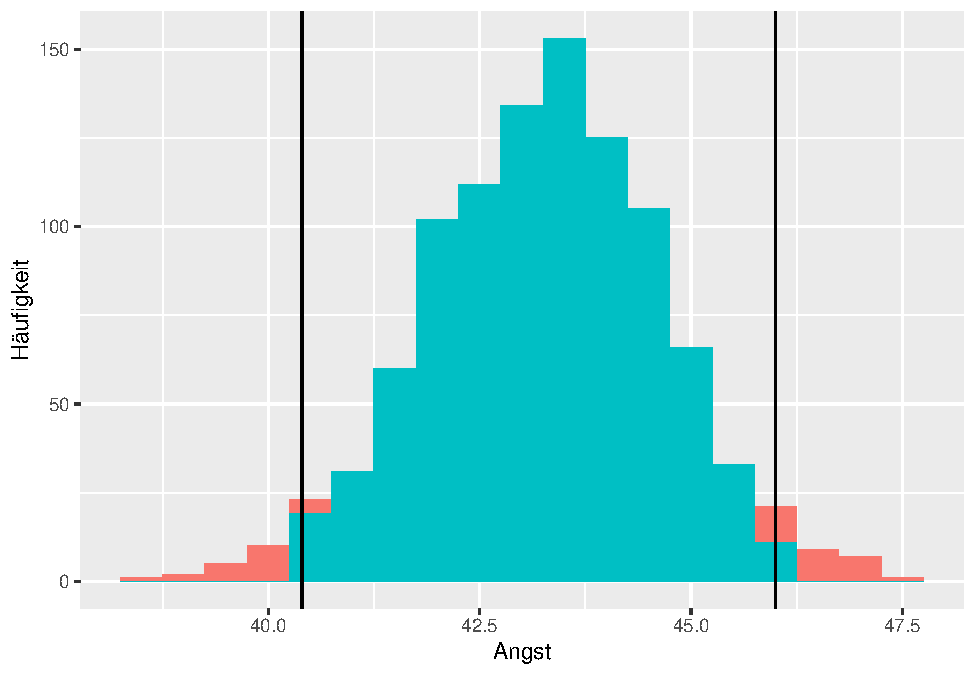
\includegraphics{aps_statistik1_files/figure-latex/exm-angst-hist-means-emp-ci-1.pdf}
\caption{\label{fig:exm-angst-hist-means-emp-ci}Verteilung der arithmetischen Mittel von 1000 zufällig gezogenen Stichproben der Angst.}
\end{figure}

\begin{example}[Verträglichkeit]
\protect\hypertarget{exm:agreableness}{}\label{exm:agreableness}Einer der Big-5 Persönlichkeitszüge ist die Verträglichkeit. Eine einfache Art die Big-5 zu messen ist mit den 10 Fragen aus dem ten-item personality inventory \emph{TIPI} \citep{gosling2003}. Für die Verträglichkeit müssen zwei Items (Item 1: Critical, quarrelsome; Item 2: Sympathetic, warm) auf einer Likert-Skala von 1 bis 7 eingeordnet werden. Anschliessend werden die Antworten gemittelt. Ein Student möchte herausfinden, ob mit diesem Messinstrument die durchschnittliche Verträglichkeit aller Menschen mittig also bei \(4\) liegt. Dafür befragt er \(n = 100\) Personen und findet die Werte \(M=3.91, s = 1.73\).
\end{example}

\begin{figure}
\centering
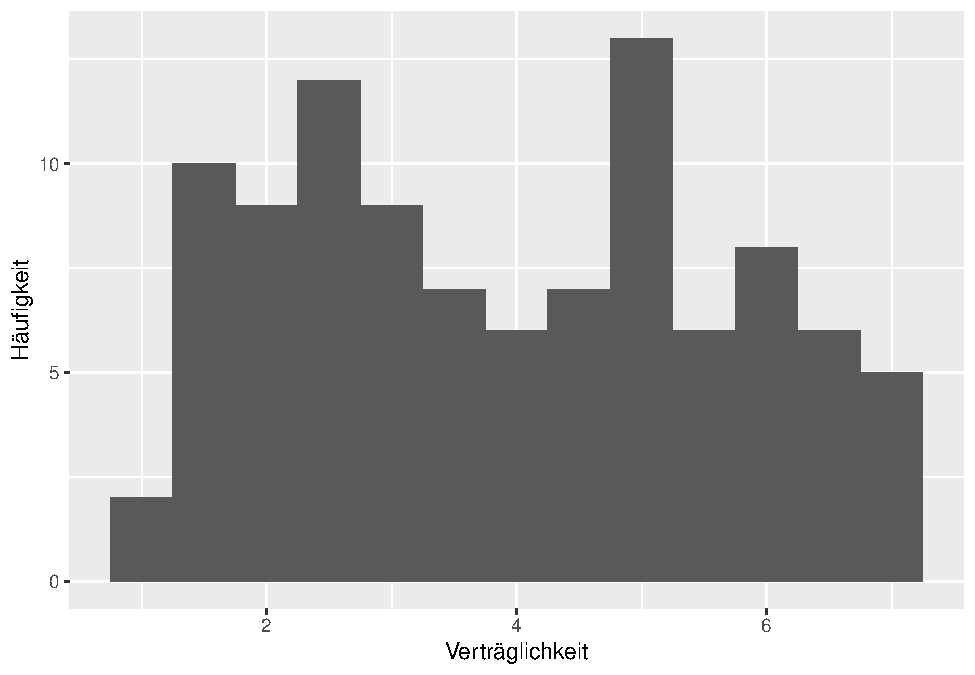
\includegraphics{aps_statistik1_files/figure-latex/exm-agreableness-hist-1.pdf}
\caption{\label{fig:exm-agreableness-hist}Verteilung der 100 beobachteten Verträglichkeitswerte einer zufällig gezogenen Stichprobe.}
\end{figure}

Die Verteilung der Beobachtungen, siehe Abbildung \ref{fig:exm-agreableness-hist}, zeigt, dass alle Werte zwischen \(1\) und \(7\) vorkommen, aber keine zentrale Tendenz greifbar ist. Um herauszufinden wie zutreffend die Schätzung des Erwartungswertes der Verträglichkeit von \(M=3.91\) ist, stelle man sich wieder vor, dass der Student \(1000\)-mal die Stichprobenziehung wiederholt und jedes mal das arithmetische Mittel \(M\) von neuem berechnet. Die Verteilung der arithmetischen Mittel dieser Stichproben ist in Abbildung \ref{fig:exm-agreableness-hist-means} dargestellt. Bei dieser Verteilung kann erneut links und rechts \(2.5\%\) der Werte abgeschnitten werden, um zum Schluss zu gelangen, dass das arithmetische Mittel in \(95\%\) der Fälle zwischen \(3.7\) und \(4.3\) zu liegen kommt.

\begin{figure}
\centering
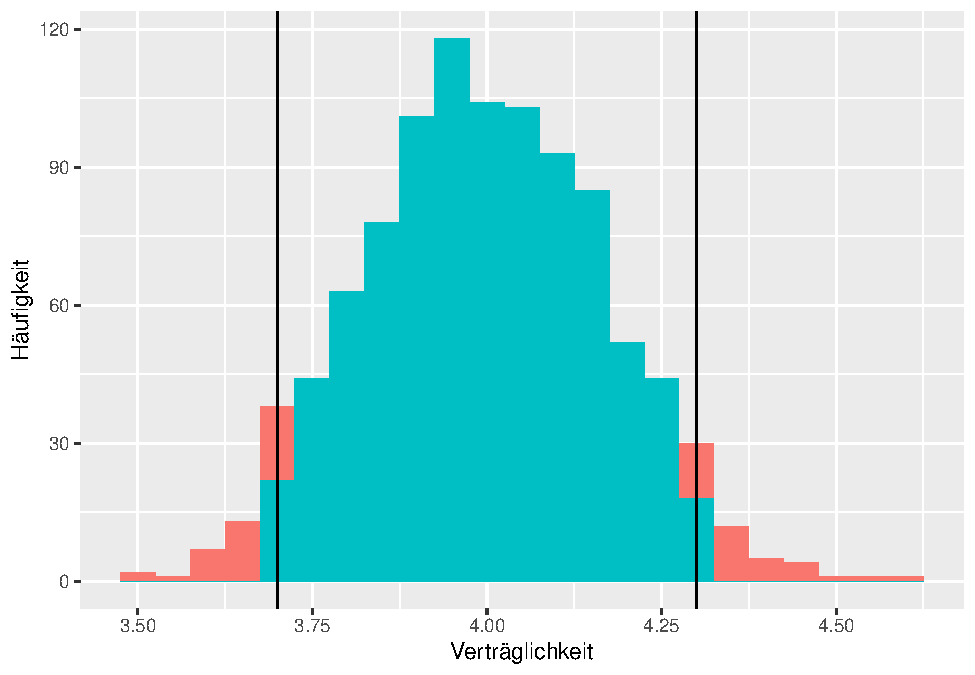
\includegraphics{aps_statistik1_files/figure-latex/exm-agreableness-hist-means-1.pdf}
\caption{\label{fig:exm-agreableness-hist-means}Verteilung der arithmetischen Mittel von 1000 zufällig gezogenen Stichproben der Verträglichkeit.}
\end{figure}

Das Problem mit diesem Vorgehen ist, dass es aus finanziellen oder technischen Gründen selten möglich ist mehrere Stichproben aus derselben Population zu ziehen. Glücklicherweise haben Statistiker:innen herausgefunden, dass die Häufigkeitsverteilungen wie in Abbildungen \ref{fig:exm-angst-hist-means-emp-ci} und \ref{fig:exm-agreableness-hist-means} immer dieselbe Verteilung haben und dies unabhängig davon wie die ursprüngliche Verteilung des Merkmals aussah. \phantomsection\label{customdef-normalverteilung}{Diese Verteilung ist eine sogenannte \textbf{Normalverteilung}}.

Die Normalverteilung sieht eine Glocke ähnlich. Deshalb wird sie auch Gausssche Glockenkurve nach Carl F. Gauss (1777-1855) benannt. Die Normalverteilung kann mit nur zwei Parametern beschrieben werden.

\begin{itemize}
\tightlist
\item
  \(\mu_g\) gibt an, wo auf der x-Achse der höchste Punkt der Glocke liegt
\item
  \(\sigma_g\) gibt an, wie flach die Glockenform ist (ein grosser Wert entspricht einer flachen Glockenform, ein tiefer Wert einer steilen Glockenform).
\end{itemize}

Auf \href{https://seeing-theory.brown.edu/probability-distributions/index.html\#section2}{seeing-theory.brown.edu \textgreater{} Continuous \textgreater{} Normal} kann der Einfluss von \(\mu\) und \(\sigma\) auf die Normalverteilung erfahren werden.

\phantomsection\label{customdef-zentraler-grenzwertsatz}{Diese Tatsache, dass die Durchschnitte aller Merkmale normalverteilt sind, ist so zentral für die Statistik, dass sie \textbf{Zentraler Grenzwertsatz} genannt wurde.} Der zentrale Grenzwertsatz besagt geneauer, dass bei einem Merkmal mit Erwartungswert \(\mu\) und Standardabweichung \(\sigma\), der Durchschnitt aller Stichprobenwerte einer Normalverteilung mit \(\mu_g = \mu\) und \(\sigma_g = \frac{\sigma}{\sqrt{n}}\) entspricht, wobei \(n\) die Stichprobengrösse bezeichnet.

\begin{caution}

\begin{remark}
\leavevmode

\begin{itemize}
\tightlist
\item
  \(\mu_g = \mu\) bedeutet, dass der Wert, welcher unter der normalverteilung am wahrscheinlichsten ist, genau dem Erwartungswert des untersuchten Merkmales entspricht.
\item
  \(\sigma_g = \frac{\sigma}{\sqrt{n}}\) hat zwei Implikationen:

  \begin{itemize}
  \tightlist
  \item
    je grösser die Streuung des Merkmals (grosses \(\sigma\)) desto breiter ist auch die Streuung der arithmetischen Mittel (grosses \(\sigma_g\)). Dies bedeutet, je weniger Streuung das Merkmal aufweist, desto genauer ist die Bestimmung des Erwartungswertes des Merkmales.
  \item
    je grösser die Anzahl Beobachtungen \(n\), desto kleiner die Streuung der arithmetischen Mittel (kleines \(\sigma_g\)). Dies bedeutet, je grösser die Stichprobe ist, desto genauer ist die Bestimmung des Erwartungswertes des Merkmales.
  \end{itemize}
\end{itemize}

\end{remark}

\end{caution}

Die Abbildungen \ref{fig:exm-angst-normal-approx} und \ref{fig:exm-agreableness-normal-approx} illustrieren den zentralen Grenzwertsatz für Beispiel \ref{exm:angst} und \ref{exm:agreableness} respektive, wobei die Normalverteilung der roten Linie entspricht. Dabei wird einstweilen angenommen, dass \(\mu\) und \(\sigma\) bekannt sind. Diese Annahme wird später aufgelöst und dient hier lediglich der Illustration.

\begin{figure}
\centering
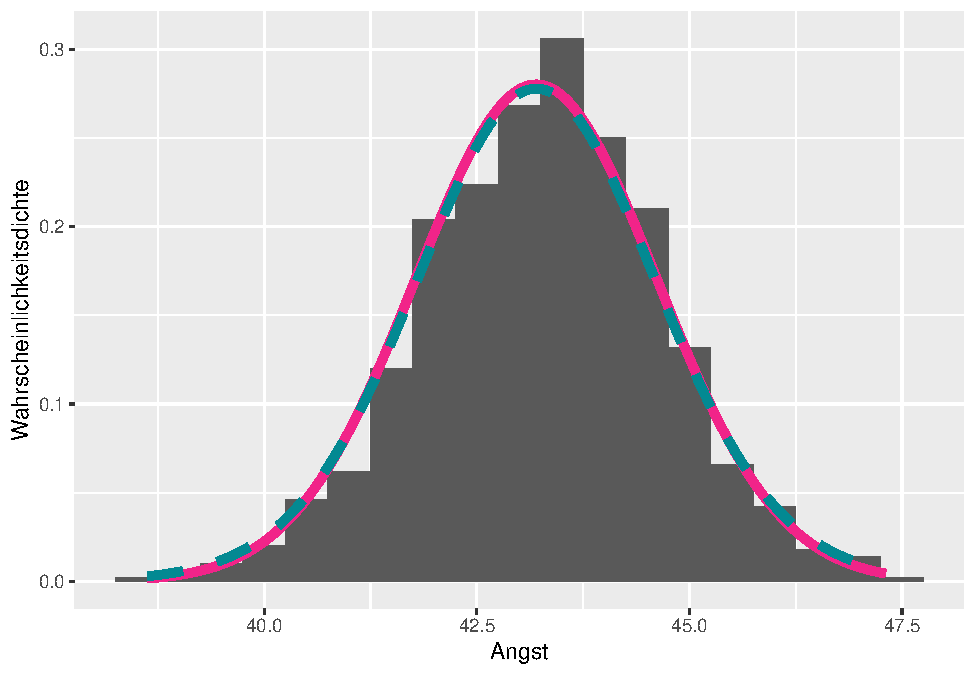
\includegraphics{aps_statistik1_files/figure-latex/exm-angst-normal-approx-1.pdf}
\caption{\label{fig:exm-angst-normal-approx}Die arithmetischen Mittel sind Normalverteilt mit Parametern \(\mu_g = 43.34\) und \(\sigma_g = 9.72 / \sqrt{30}\).}
\end{figure}

\begin{figure}
\centering
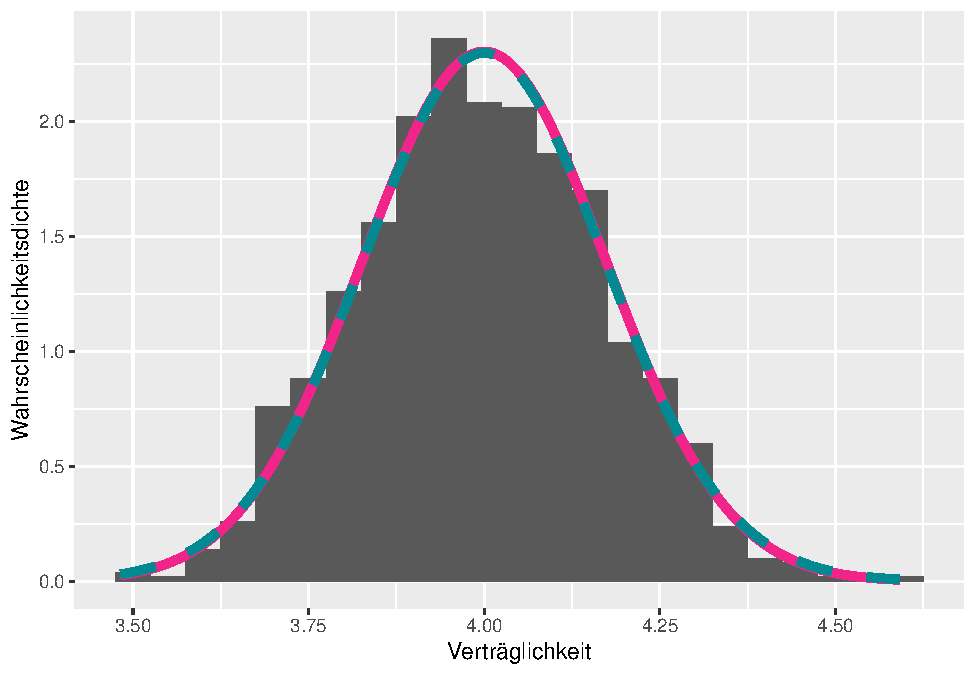
\includegraphics{aps_statistik1_files/figure-latex/exm-agreableness-normal-approx-1.pdf}
\caption{\label{fig:exm-agreableness-normal-approx}Die arithmetischen Mittel sind Normalverteilt mit Parametern \(\mu_g = 3.91\) und \(\sigma_g = 1.73 / \sqrt{100}\).}
\end{figure}

Die Erkenntnis des zentralen Grenzwertsatz macht also das wiederholte ziehen von Stichproben unnötig. Die Normalverteilung ist theoretisch konstruiert und ihr \(2.5\%\)- und \(97.5\%\)-Perzentil können theoretisch hergeleitet werden. Tabelle \ref{tab:quantiles-norm} wird kann beobachtet werden, dass für unsere zwei Beispiele die Perzentile der Stichprobe und der Normalverteilung sehr ähnlich, wenn auch nicht exakt gleich sind. Die Ungenauigkeit rührt daher, dass der zentrale Grenzwertsatz nur dann exakt funktioniert, wenn die Anzahl Beobachtungen (unendlich) gross ist.

\begin{table}
\centering
\caption{\label{tab:quantiles-norm}Vergleich Perzentile der Stichprobe und der theoretischen Verteilung.}
\centering
\begin{tabular}[t]{crrrrcr}
\toprule
\multicolumn{1}{c}{ } & \multicolumn{2}{c}{Stichprobe} & \multicolumn{2}{c}{Normalverteilung} & \multicolumn{2}{c}{t-Verteilung} \\
\cmidrule(l{3pt}r{3pt}){2-3} \cmidrule(l{3pt}r{3pt}){4-5} \cmidrule(l{3pt}r{3pt}){6-7}
Beispiel & 2.5\% & 97.5\% & 2.5\% & 97.5\% & 2.5\% & 97.5\%\\
\midrule
Angst & 40.4 & 46.0 & 42.23 & 44.46 & 42.18 & 44.50\\
Vertraeglichkeit & 3.7 & 4.3 & 3.66 & 4.34 & 3.66 & 4.34\\
\bottomrule
\end{tabular}
\end{table}

Einstweilen wurde hier angenommen, dass die Streuung des Merkmals \(\sigma\) bekannt ist. Dies ist in der Realität nie der Fall und eine weitere, wenn auch weniger grosse Ungenauigkeitsquelle. \phantomsection\label{customdef-student-verteilung}{Wenn \(\sigma\) also auch aus der Stichprobe geschätzt werden muss, ist die Ännäherung der Verteilung der arithmetischen Mittel besser gegeben mit einer \textbf{Student-\(t\)-Verteilung} oder kurz \(t\)-Verteilung.} Die grüne gestrichtelte Linie in den Abbildungen \ref{fig:exm-angst-normal-approx} und \ref{fig:exm-agreableness-normal-approx} entspricht der \(t\)-Verteilung im jeweiligen Beispiel.

Der Unterschied zwischen der Normalverteilung und der \(t\)-Verteilung ist nur sichtbar, wenn \(n\) klein ist. In Beispiel \ref{exm:angst} mit \(n = 30\) ist ein kleiner Unterschied, in Beispiel \ref{exm:agreableness} mit \(n = 100\) ist kein Unterschied zwischen der Normalverteilung und der \(t\)-Verteilung sichtbar. \phantomsection\label{customdef-freiheitsgrade}{Tatsächlich wird die \(t\)-Verteilung mit einem Parameter charaktisiert, welcher \textbf{Freiheitsgrade} (eng. degrees of freedom, \(df\)) genannt wird.} In Abbildung \ref{fig:t-distribution} wird die \(t\)-Verteilung mit verschiedenen Freiheitsgraden mit der Normalverteilung verglichen. Bei der \(t\)-Verteilung mit den kleinsten Freiheitsgraden sind extremere Werte wahrscheinlicher als \(t\)-Verteilungen mit grösseren Freiheitsgraden.

\begin{figure}
\centering
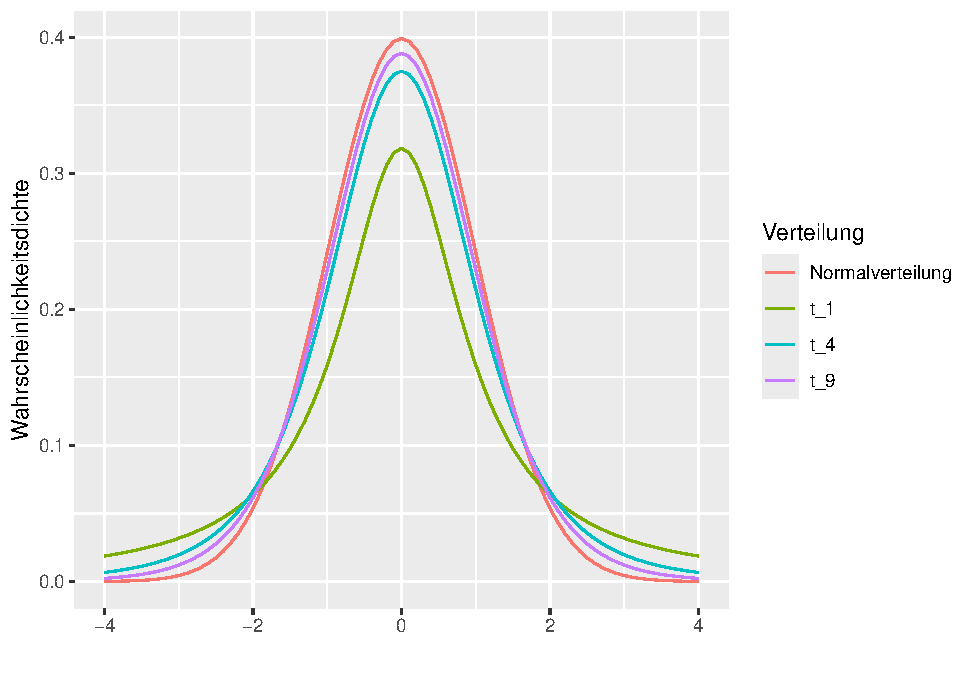
\includegraphics{aps_statistik1_files/figure-latex/t-distribution-1.pdf}
\caption{\label{fig:t-distribution}Student-t-Verteilungen mit 1, 4 und 9 Freiheitsgraden im Vergleich zu der Normalverteilung.}
\end{figure}

Die Freiheitsgrade der \(t\)-Verteilung in der Annäherung oben entsprechen der Anzahl Beobachtungen minus 1, also \(df = n-1\). Die höhere Wahrscheinlichkeit von extremeren Werten bei kleinen Freiheitsgraden spiegelt die grössere Unsicherheit der Schätzung des Erwartungswertes wieder, wenn die Standardabweichung unbekannt und damit auch geschätzt werden muss. Je kleiner \(n\) ist, desto stärker fällt diese Unsicherheit aus.

Die arithmetischen Mittel bei unbekannter Standardabweichung sind bei wiederholter Stichprobenziehung genau \(t\)-verteilt. Um die Genauigkeit der Schätzung des Erwartungswertes zu bestimmen genügt es folglich, das 2.5\% und das 97.5\% Perzentil der \(t\)-Verteilung mit \(n-1\) Freiheitsgraden zu bestimmen. Diese Perzentile können mit

\[ \bar{x} - \frac{s}{\sqrt{n}} \cdot t_{97.5\%, n-1} < \mu < \bar{x} + \frac{s}{\sqrt{n}} \cdot t_{97.5\%, n-1}\]

berechnet werden, wobei \(\bar{x}\) das arithmetische Mittel, \(s\) die Standardabweichung und \(t_{97.5\%, n-1}\) dem Wert des 97.5\%-Perzentil einer auf 0 zentrierten \(t\)-Verteilung mit \(n-1\) Freiheitsgraden entspricht. Letzere Perzentile der \(t\)-Verteilung können bei Bedarf in entsprechenden Tabellen nachgeschlagen werden. Als Gedankenstütze kann für \(t_{97.5\%, n-1}\) immer \(2\) gedacht werden, da dies ungefähr dem wahren Wert entspricht, wenn \(n\) grösser als \(50\) ist.

Das \(2.5\%\) und das \(97.5\%\) Perzentil der Verteilung der arithmetischen Mittel ergeben nun die untere respektive obere Schranke eines \phantomsection\label{customdef-interval}{\textbf{Intervalles}. Ein Intervall bezeichnet durch die Symbolik \([\)untere Schranke, obere Schranke\(]\) beinhaltet alle Zahlen zwischen der unteren und der oberen Schranke.} \phantomsection\label{customdef-confidence-interval}{Ein Intervall mit den oben beschriebenen Perzentilen als Schranken wurde so berechnet, dass bei wiederhohlter Stichprobenziehung der wahre Erwarungswert in \(95\%\) der Fälle umschlossen wird. Grob übersetzt bedeutet dies, dass wir zu \(95\%\) sicher oder \emph{konfident} sind, dass der Erwarungswert in diesem Intervall liegt. Dieses Intervall wird deshalb als \(95\%\)-\textbf{Konfidenzintervall} (symbol KI) bezeichnet.}

In Beispiel \ref{exm:angst}, kann aus der Tabelle \ref{tab:quantiles-norm} entnommen werden, dass die Angst in der Population bei \(M = 43.34\) \(95\%\) KI \([42.18,44.5]\) liegt. In Beispiel \ref{exm:agreableness}, kann aus der Tabelle \ref{tab:quantiles-norm} entnommen werden, dass die Verträglichkeit in der Population bei \(M = 3.91\) \(95\%\) KI \([3.66,4.34]\) liegt. Wann immer eine Schätzung eines zentralen Wertes berichtet wird, soll dies ab jetzt in der soeben gezeigten Darstellung inklusive Angabe des Konfidenzintervalls erfolgen. Damit wird der Leserin aufgezeigt, wo der Schätzwert der zentralen Tendenz liegt und gleichzeigtig wird intuitiv vermittelt wie genau die Schätzung ist.

Es ist nun spannend zu explorieren, wie sich die Stichprobengrösse \(n\) oder die geschätzte Standardabweichung \(s\) auf die Länge des Konfidenzintervalls auswirkt. Dies kann in den Übungen \ref{exr:ki-mean-n-vary} und \ref{exr:ki-mean-s-vary} selbst erforscht werden.

\section{Übungen}\label{uxfcbungen-1}

\begin{exercise}
\protect\hypertarget{exr:interpret-report1}{}\label{exr:interpret-report1}\leavevmode

\begin{verbatim}
## [1] "hi"
\end{verbatim}

\end{exercise}

\begin{solution}
TODO
\end{solution}

\begin{exercise}
\protect\hypertarget{exr:interpret-report2}{}\label{exr:interpret-report2}\leavevmode

\begin{verbatim}
## [1] "hi"
\end{verbatim}

\end{exercise}

\begin{solution}
TODO
\end{solution}

\begin{exercise}
\protect\hypertarget{exr:ki-approx-normal}{}\label{exr:ki-approx-normal}\leavevmode

Für ein Experiment werden in drei Runden jeweils \(10000\) Zufallsstichproben erhoben mit respektive \(10\), \(40\) und \(100\) Beobachtungen pro Zufallsstichprobe. Die Verteilung der jeweils ersten Zufallsstichprobe für eine Stichprobengrösse ist in Abbildung \ref{fig:ki-approx-normal1} dargestellt. Die Daten sind nicht normalverteilt, weil keine Glockenkurve wie oben beschrieben das Histogramm gut abdecken würde.

\begin{figure}
\centering
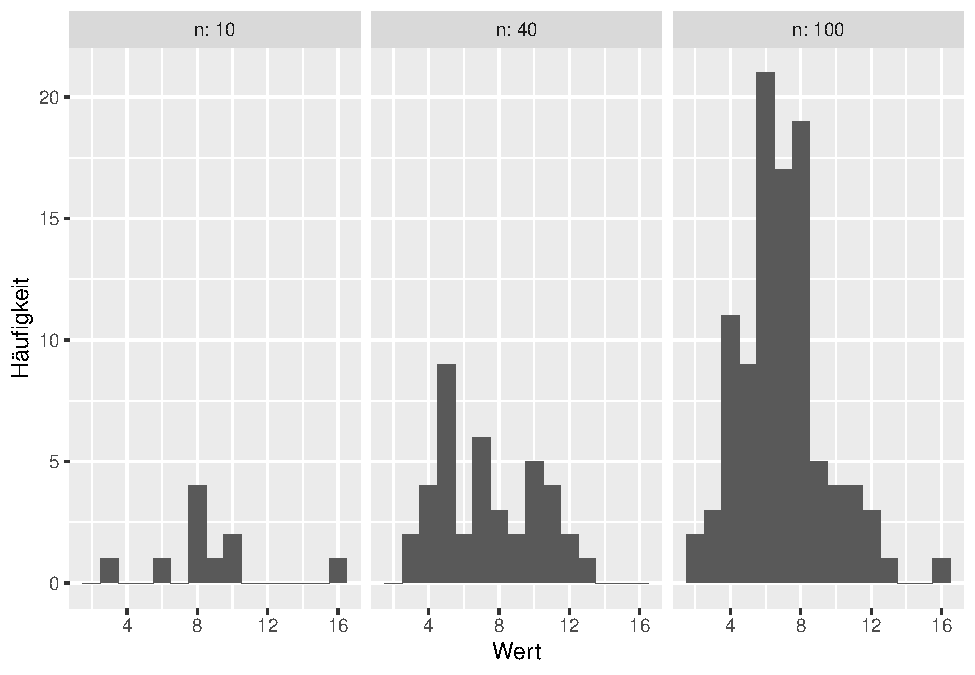
\includegraphics{aps_statistik1_files/figure-latex/ki-approx-normal1-1.pdf}
\caption{\label{fig:ki-approx-normal1}TODO.}
\end{figure}

Die arithmetischen Mittel der 10'000 Stichproben sind im Datensatz \texttt{04-exr-zentraler-grenzwertsatz.sav} festgehalten. In der Spalte \texttt{n\_10} zum Beispiel steht jede Zeile für das arithmetische Mittel eine Zufallstichprobe mit 10 Beobachtungen. Der zentrale Grenzwertsatz besagt, dass diese arithmetischen Mittel normalverteilt sind mit zunehmender Stichprobengrösse \(n\). Erstellen Sie ein Histogramm mit der Erweiterung \texttt{JJStatsPlot} und zeichnen Sie eine Normalverteilung darüber. Interpretieren Sie das Resultat.

\end{exercise}

\begin{solution}

Die Übereinanderlegung des jeweiligen Histograms und der Wahrscheinlichkeitsdichte der Normalverteilung wird in Abbildung \ref{fig:sol-ki-approx-normal} gezeigt. Es ist deutlich zu sehen, dass die Linie nur bei \(n=100\) die Häufigkeitsverteilung der arithmetischen Mittel gut nachbilden kann. Bei \(n=10\) und \(n=50\) ist ein grosser Unterschied zwischen Häufigkeitsverteilung und Linie sichtbar. Das genaue \(n\) ab welchem eine Häufigkeitsverteilung gut durch die Normalverteilung angenähert wird hängt von der ursprünglichen Verteilung der Daten ab, d.h. der Verteilung in Abbildung \ref{fig:ki-approx-normal1}. Es kann deshalb nicht generell gesagt werden, dass ab \(n=100\) die Annäherung immer gut sei, so wie in diesem Beispiel. Der zentrale Grenzwertsatz besagt demnach auch lediglich, dass man immer ein grosses \(n\) wählen kann, so dass die Annäherung gut ist. Er besagt nichts darüber, wie gross \(n\) sein muss.

\begin{figure}
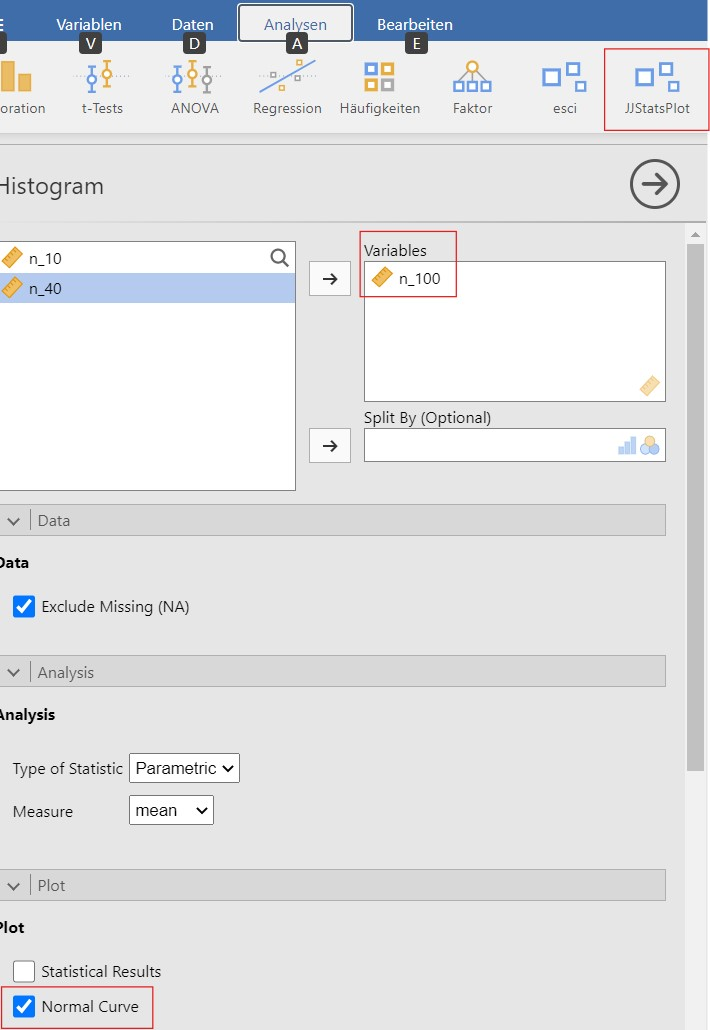
\includegraphics[width=0.5\linewidth]{figures/04-exr-ki-approx-normal-jmv-input} 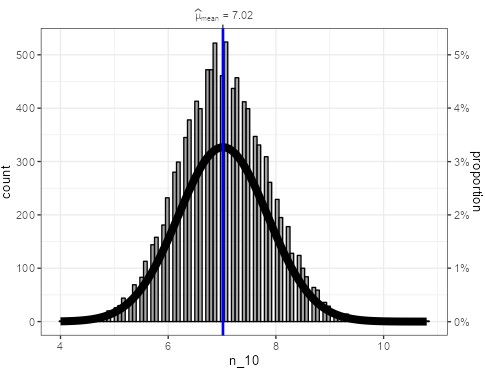
\includegraphics[width=0.5\linewidth]{figures/04-exr-ki-approx-normal-jmv-output1} 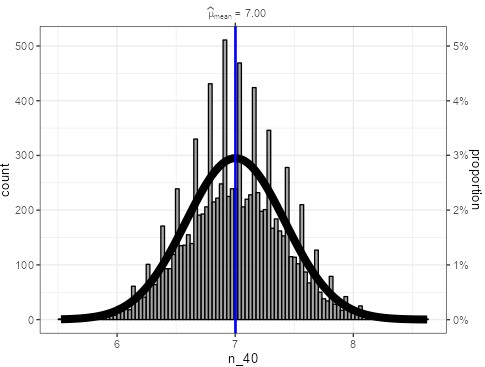
\includegraphics[width=0.5\linewidth]{figures/04-exr-ki-approx-normal-jmv-output2} 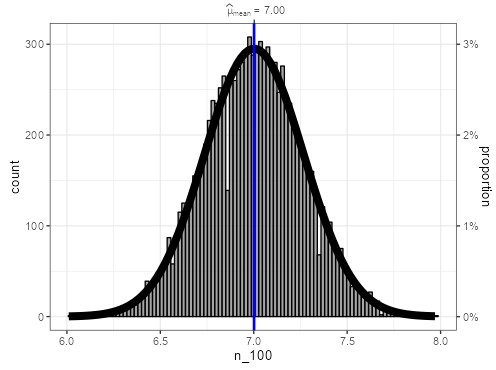
\includegraphics[width=0.5\linewidth]{figures/04-exr-ki-approx-normal-jmv-output3} \caption{TODO}\label{fig:sol-ki-approx-normal}
\end{figure}

\end{solution}

\begin{exercise}
\protect\hypertarget{exr:ki-mean-n-vary}{}\label{exr:ki-mean-n-vary}\leavevmode

Eine Mensa will herausfinden, wie lange die Leute um 12h durchschnittlich anstehen müssen. Dazu befragt sie 5 Kund:innen. Das Resultat der Untersuchung ist, dass die Kund:innen im Durchschnitt \(0.4\) Stunden anstehen müssen. Leider ist das Konfidenzintervall sehr gross. Da die Mensa nicht weiss, wie viele Leute befragt werden müssen, um ein kleineres Konfidenzintervall zu erhalten befragt sie in 4 weiteren Runden jeweils 20, 50, 100 und 1000 Kund:innen. Die Daten aller 5 Untersuchungen sind unter \texttt{04-exr-stichprobengroesse.sav} abgelegt. Für jede der 5 Stichproben:

\begin{enumerate}
\def\labelenumi{\alph{enumi}.}
\tightlist
\item
  Was ist die Schätzung des Erwartungswertes der Wartezeit?
\item
  Wie gross ist die Standardabweichung der Wartezeit?
\item
  Wie gross ist die Standardabweichung der arithmetischen Mittel?
\item
  Bestimmen Sie die 95\%-Konfidenzintervalle.
\item
  Berechnen Sie die Länge jedes Konfidenzintervalls.
\end{enumerate}

Vergleichen Sie die Resultate der Berechnungen für jede Stichprobe:

\begin{enumerate}
\def\labelenumi{\alph{enumi}.}
\setcounter{enumi}{5}
\tightlist
\item
  Weshalb ist die Schätzung für den Erwartungswert für jede Stichprobe unterschiedlich?
\item
  Was lässt sich über den Zusammenhang zwischen Stichprobengrösse und der Länge des Konfidenzintervalls sagen?
\end{enumerate}

\end{exercise}

\begin{solution}

Abbildung \ref{fig:sol-ki-mean-n-vary} zeigt die Berechnunganweisungen für Jamovi und die resultierende Tabelle daraus.

\begin{figure}
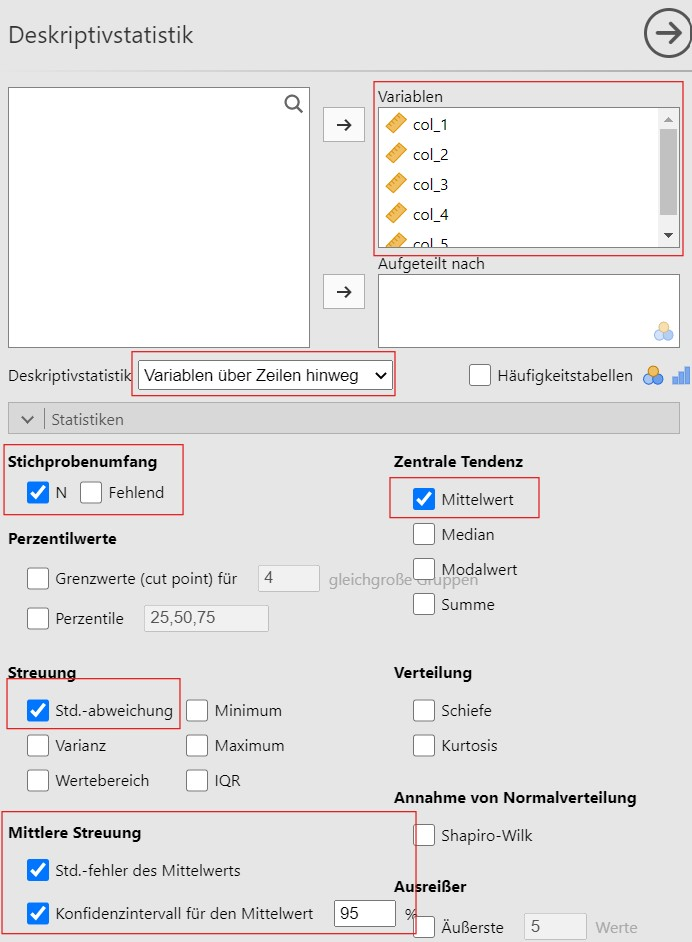
\includegraphics[width=0.5\linewidth]{figures/04-exr-stichprobengroesse-jmv-input} 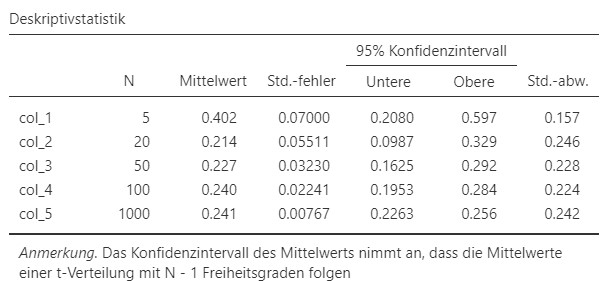
\includegraphics[width=0.5\linewidth]{figures/04-exr-stichprobengroesse-jmv-output} \caption{Links: Jamovi-Anleitung zur Erstellung der Tabelle mit den relevanten Kenngrössen; rechts: Tabelle mit relevanten Kenngrössen.}\label{fig:sol-ki-mean-n-vary}
\end{figure}

\begin{enumerate}
\def\labelenumi{\alph{enumi}.}
\tightlist
\item
  Der Erwartungswert der Wartezeiten (das heisst der Populationmittelwerte der Wartezeiten) wird mit dem arithmetischen Mittel der Stichprobe geschätzt und kann in der Tabelle bei \texttt{Mittelwert} abgelesen werden. Der Erwartungswert der Wartezeiten beträgt bei allen Stichproben ausser bei der ersten ungefähr 0.22 Stunden, also ein bisschen weniger als eine Viertelstunde.
\item
  Der Standardabweichung der Wartezeiten der Stichprobe sind in der Tabelle bei \texttt{Std.-abw.} abzulesen. Die Standardabweichungen sind für alle Stichproben ausser der ersten ungefähr bei 0.23.
\item
  Die Standardabweichung der arithmetischen Mittel liegt bei \(s/\sqrt{n}\). Für die erste Stichprobe ist dies \(0.157 / \sqrt{5} = 0.0702125\). Diese Werte werden auch als Standardfehler bezeichnet und sind in der Tabelle bei \texttt{Std.-fehler} ablesbar.
\item
  Die untere und obere Schranke der 95\%-Konfidenzintervalle sind bei \texttt{Untere} und \texttt{Obere} respektive abzulesen.\\
\item
  Die Länge des Konfidenzintervalls entspricht jeweils dem höheren Wert minus dem tieferen Wert. Für die erste Stichprobe ist dies 0.597 - 0.208 = 0.389, für die anderen 0.23, 0.13, 0.09 und 0.03.
\item
  Die Schätzung des Erwartungswertes ist das arithmetische Mittel der Stichprobe. Da jedesmal eine neue Zufallsstichprobe gezogen wurde und diese nicht dieselben Beobachtungen enthalten, ergeben sich auch jedesmal andere Stichprobenmittelewerte.
\item
  Je grösser \(n\), desto kleiner ist das Konfidenzintervall. Wenn man also ein kleines Konfidenzintervall erreichen will, braucht man eine grössere Stichprobe.
\end{enumerate}

\end{solution}

\begin{exercise}
\protect\hypertarget{exr:ki-mean-s-vary}{}\label{exr:ki-mean-s-vary}\leavevmode

\begin{verbatim}
## [1] "hi"
\end{verbatim}

\end{exercise}

\begin{solution}
TODO
\end{solution}

\chapter{Zentrale Tendenz testen}\label{zentrale-tendenz-testen}

Eine andere Fragestellung, die mit Daten oft beantwortet wird ist, ob eine gewisse Aussage wahr ist oder falsch. \phantomsection\label{customdef-hypothese}{Eine solche Aussage wird \textbf{Hypothese} (Symbol: \(H\)) genannt.} Eine Hypothese könnte zum Beispiel sein:

\begin{quote}
\(H:\) Es regnet.
\end{quote}

Ist die Hypothese einmal gefunden, können Daten gesammelt werden, um diese Hypothese zu bestätigen oder zu falsifizieren. Man geht nach draussen und spürt Regen auf der Haut bedeutet \(H\) ist wahr, spürt man keinen Regen, so ist \(H\) falsch.

Wenn eine Hypothese wahr ist, dann ist das Gegenteil der Hypothese falsch. Weil oft über die Hypothese und ihr Gegenteil debattiert wird, ist es nützlich die beiden auch terminologisch auseinanderhalten zu können. \phantomsection\label{customdef-nullhypothese}{Die Hypothese, welche den bisherigen Informationsstand reflektiert wird \textbf{Nullhypothese} (Symbol \(H_0\)) genannt.} War es draussen bei der letzten Messung vor einer Stunde schönes Wetter, dann ist die Nullhypothese

\begin{quote}
\(H_0:\) Es regnet nicht.
\end{quote}

\phantomsection\label{customdef-alternativhypothese}{Das Gegenteil der Nullhypothese wird \textbf{Alternativhypothese} (Symbol \(H_1\)) genannt.} Im Beispiel ist die Alternativhypothese

\begin{quote}
\(H_1:\) Es regnet.
\end{quote}

\section{Entspricht der Erwartungswert einem gewissen Wert?}\label{entspricht-der-erwartungswert-einem-gewissen-wert}

Um eine Hypothese mit Daten überprüfbar zu machen, muss diese in eine Form gebracht werden, welche Daten einbezieht. Eine einfache Form einer solchen überprüfbaren Hypothese ist

\begin{quote}
\(H:\) Das durchschnittliche Vermögen einer in der Schweiz lebenden Person beträgt \(100'000\) CHF.
\end{quote}

Wenn die Population alle in der Schweiz lebenden Personen sind, dann entspricht dies also der Nullhypothese

\begin{quote}
\(H_0:\mu = 100'000\).
\end{quote}

Abstrahiert, soll bei dieser Problemstellung herausgefunden werden, ob der Erwartungswert einer Population einem gewissen Wert entspricht. Das Gegenteil dieser Nullhypothese ist die Alternativhypothese

\begin{quote}
\(H_1: \mu \neq 100'000\).
\end{quote}

Dies bedeutet, dass das Vermögen der Population nicht bei \(100'000\) CHF liegt. \phantomsection\label{customdef-zweiseitige-hypothese}{Weil die Alternativhypothese hier zwei Ausgänge zulässt, nämlich kleiner oder grösser als \(100'000\) CHF wird diese Art \textbf{zweiseitige Hypothese} bezeichnet.}

Eine weitere Form der Hypothese wäre

\begin{quote}
\(H:\) Das durchschnittliche Vermögen einer in der Schweiz lebenden Person beträgt weniger als oder genau \(100'000\) CHF.
\end{quote}

In Formelsprache übersetzt entspricht dies

\begin{quote}
\(H_0: \mu \leq 100'000\).
\end{quote}

Das Gegenteil davon ist, wenn das durchschnittliche Vermögen grösser und ungleich 100'000 CHF ist, also

\begin{quote}
\(H_1: \mu > 100'000\).
\end{quote}

\begin{caution}

\begin{remark}

Die verwendeten Zeichen in den Formeln sind

\begin{itemize}
\tightlist
\item
  \(=\): Gleichheit, sprich ``gleich''. Beispiele:

  \begin{itemize}
  \tightlist
  \item
    \(3 = 3\) (\(3\) gleich \(3\)) ist eine wahre Aussage.
  \item
    \(3 = 4\) (\(3\) gleich \(4\)) ist eine falsche Aussage.
  \end{itemize}
\item
  \(\neq\): Ungleichheit, sprich ``ungleich'' oder ``nicht gleich''. Beispiele:

  \begin{itemize}
  \tightlist
  \item
    \(3 \neq 3\) (\(3\) ist nicht gleich \(3\)) ist eine falsche Aussage.
  \item
    \(3 \neq 4\) (\(3\) ist nicht gleich \(4\)) ist eine wahre Aussage.
  \end{itemize}
\item
  \(<\): Kleiner, sprich ``kleiner''. Beispiele:

  \begin{itemize}
  \tightlist
  \item
    \(4 < 3\) (\(4\) ist kleiner als \(3\)) ist eine falsche Aussage.
  \item
    \(3 < 3\) (\(3\) ist kleiner als \(3\)) ist eine falsche Aussage.
  \item
    \(3 < 4\) (\(3\) ist kleiner als \(4\)) ist eine wahre Aussage.
  \end{itemize}
\item
  \(\leq\): Kleiner gleich, sprich ``kleiner gleich''. Beispiele:

  \begin{itemize}
  \tightlist
  \item
    \(4 \leq 3\) (\(4\) ist kleiner oder gleich wie \(3\)) ist eine falsche Aussage.
  \item
    \(3 \leq 3\) (\(3\) ist kleiner oder gleich wie \(3\)) ist eine wahre Aussage.
  \item
    \(3 \leq 4\) (\(3\) ist kleiner oder gleich wie \(4\)) ist eine wahre Aussage.
  \end{itemize}
\item
  \(>\): Grösser, sprich ``grösser''. Beispiele:

  \begin{itemize}
  \tightlist
  \item
    \(4 > 3\) (\(4\) ist grösser als \(3\)) ist eine wahre Aussage.
  \item
    \(3 > 3\) (\(3\) ist grösser als \(3\)) ist eine falsche Aussage.
  \item
    \(3 > 4\) (\(3\) ist grösser als \(4\)) ist eine falsche Aussage.
  \end{itemize}
\item
  \(\geq\): Grösser gleich, sprich ``grösser gleich''. Beispiele:

  \begin{itemize}
  \tightlist
  \item
    \(4 \geq 3\) (\(4\) ist grösser oder gleich wie \(3\)) ist eine wahre Aussage.
  \item
    \(3 \geq 3\) (\(3\) ist grösser oder gleich wie \(3\)) ist eine wahre Aussage.
  \item
    \(3 \geq 4\) (\(3\) ist grösser oder gleich wie \(4\)) ist eine falsche Aussage.
  \end{itemize}
\end{itemize}

\end{remark}

\end{caution}

\begin{example}[Vermögen]
\protect\hypertarget{exm:vermoegen}{}\label{exm:vermoegen}\leavevmode

Eine Sozialpolitikberatungsfirma will herausfinden, ob das durchschnittliche Vermögen der in der Schweiz lebenden Personen im letzten Jahr gestiegen ist. Sie stellen dazu basierend auf dem aktuellen Wissensstand die Nullhypothese auf, dass das durchschnittliche Vermögen nicht gestiegen ist, und die Alternativhypothese, dass das durchschnittliche Vermögen gestiegen ist:

\begin{quote}
\(H_0: \mu \leq 100'000\) CHF
\end{quote}

\begin{quote}
\(H_1: \mu > 100'000\) CHF
\end{quote}

Um die Hypothesen auf einer Datengrundlage zu evaluieren, erfragt es das Vermögen von \(n=20\) zufällig ausgewählten Personen und findet ein durchschnittliches Vermögen von \(M=119853\) CHF.

\end{example}

Es kann nun schnell gesagt werden, dass das durchschnittliche Vermögen in der Population gestiegen ist, weil \(193'000\) CHF grösser ist als \(100'000\) CHF. Dies so zu behaupten wäre jedoch falsch, weil nicht alle Personen in der Population befragt wurden, sondern lediglich eine Zufallsstichprobe. Wie in Kapitel \ref{stichprobenziehung} muss hier für eine Generalisierung der Stichprobe auf die Population der Effekt der zufälligen Stichprobenziehung miteinbezogen werden.

Aufgrund der Zufallsstichprobe ist es unmöglich zu sagen, ob unsere Stichprobe eine eher seltene Stichprobenziehung aus einer Population mit unverändertem durchschnittlichen Vermögen von \(100'000\) CHF ist (Abbildung \ref{fig:exm-vermoegen-sampling-plot} links) oder ob es eine eher häufig vorkommende Stichprobenziehung aus einer Population mit höherem durchschnittlichen Vermögen ist (Abbildung \ref{fig:exm-vermoegen-sampling-plot} rechts).

\begin{figure}
\centering
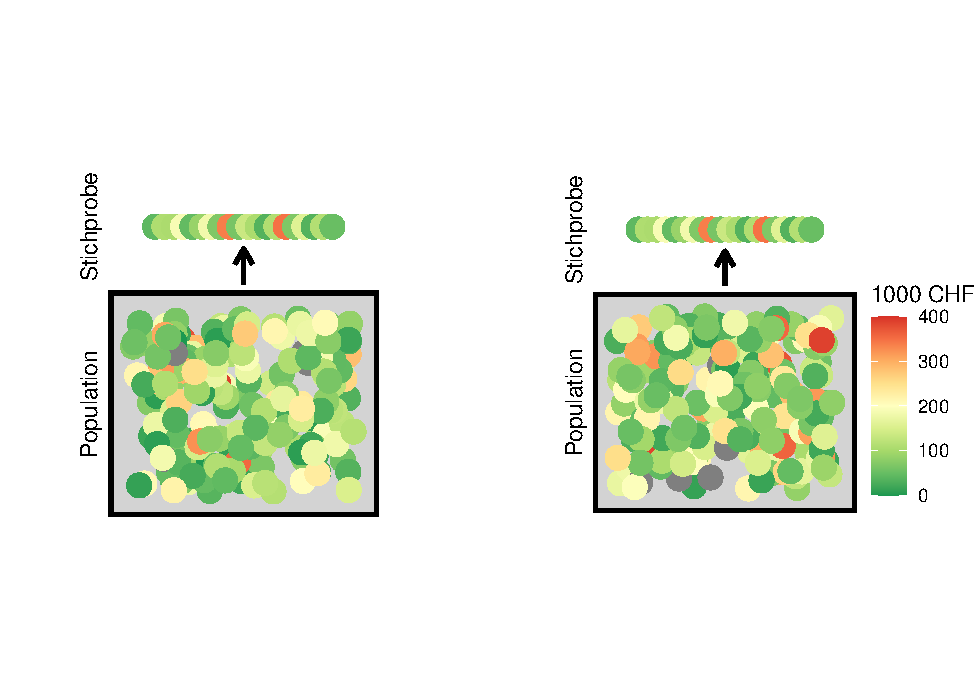
\includegraphics{aps_statistik1_files/figure-latex/exm-vermoegen-sampling-plot-1.pdf}
\caption{\label{fig:exm-vermoegen-sampling-plot}Vorgestellte Zufallsstichprobenziehung. Links: Nullhypothese ist wahr. Rechts: Nullhypothese ist falsch.}
\end{figure}

Es kann jedoch ausgesagt werden, mit welcher Wahrscheinlichkeit der gefundene Stichprobenmittelwert realisiert wird, gegeben dass die Nullhypothese wahr ist. Hier wird also angenommen, dass eine Population mit Erwartungswert \(\mu = 100'000\) CHF vorliegt und dass anschliessend zum Beispiel \(3000\) Stichproben an je \(20\) Beobachtungen pro Stichprobe gezogen werden. Von jeder dieser Stichproben wird das arithmetische Mittel berechnet. In der Verteilung dieser Mittelwerte, siehe Abbildung \ref{fig:exm-vermoegen-histogram-plot}, wird nun der tatsächliche Mittelwert der Stichprobe \(\bar{x} = 119853\) verortet.

\begin{figure}
\centering
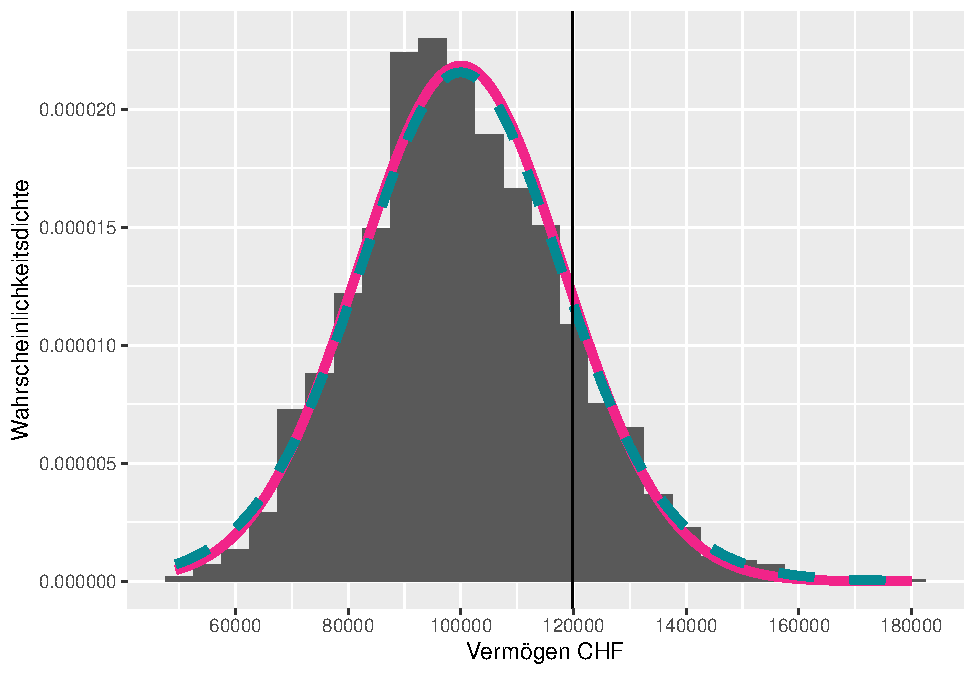
\includegraphics{aps_statistik1_files/figure-latex/exm-vermoegen-histogram-plot-1.pdf}
\caption{\label{fig:exm-vermoegen-histogram-plot}TODO.}
\end{figure}

Der beobachtete Mittelwert ist zwar nicht genau bei \(100'000\) CHF, aber trotzdem noch einigermassen plausibel, wenn die Nullhypothese stimmt. Um diesen Gedanken zu formalisieren, gibt es zwei Denkweisen, welche nun vorgestellt werden.

Die eine von Ronald Fisher Denkweise ist die Frage nach der Wahrscheinlichkeit, dass der beobachtete Wert oder ein noch extremerer Wert in Richtung der Alternativhypothese resultiert. Im Beispiel entspricht dies der Wahrscheinlichkeit den Wert \(119853\) oder einen grösseren Wert zu beobachten, wenn der Erwartungswert tatsächlich bei \(100'000\) CHF liegt. Um diese Wahrscheinlichkeit zu bestimmen, kann einfach gezählt werden, welcher Anteil der Stichprobenmittel werte grösser oder gleich \(119853\) CHF ist. Im Beispiel sind dies \(0.143 = 14.3\%\). \phantomsection\label{customdef-pwert}{Dieser Wert wird, abgeleitet vom englischen \emph{probability} auch \textbf{p-Wert} (Symbol: \(p\)) genannt. Beim Berichten des p-Werts wird normalerweise die führende \(0\) nicht geschrieben, also \(p = .143\).}

\phantomsection\label{customdef-signifikanzniveau}{Bei der anderen Denkweise muss noch vor der Datenerhebung ein sogenanntes \textbf{Signifikanzniveau} (Symbol \(\alpha\), sprich `alpha') bestimmt werden. Dieser Wert entspricht der Wahrscheinlichkeit, dass der statistische Test die Nullhypothese verwirft, obwohl diese wahr gewesen wäre. Normalerweise wird \(\alpha = 5\%\) gesetzt.} Es wird also akzeptiert, dass ein statistischer Test in \(5\%\) der Fälle gegen die Nullhypothese entscheidet, obwohl diese wahr wäre. \phantomsection\label{customdef-ablehnungsbereich}{In einem zweiten Schritt wird bestimmt, welches die \(5\%\) unwahrscheinlichsten Werte sind, wenn die Nullhypothese wahr ist. Diese Werte werden \textbf{Ablehnungsbereich} genannt.} Im Beispiel sind dies die \(5\%\) höchsten Werte, nämlich Vermögen von \(131511\) CHF und grössere Vermögen. Nun wird bestimmt, ob der tatsächliche beobachtete Wert im Ablehnungsbereich liegt oder nicht. \phantomsection\label{customdef-signifikanz}{Im Beispiel liegt der Stichprobenmittelwert \(119853\) CHF nicht im Ablehnungsbereich. In diesem Fall wird die Nullhypothese nicht verworfen und das Testresultat erhält das Prädikat \textbf{nicht signifikant}. Läge der Stichprobenmittelwert im Ablehnungsbereich, so wäre das Testresultat als \textbf{signifikant} einzustufen.}

\begin{caution}

\begin{remark}
Ein signifikanter Unterschied bedeutet im allgemeinen Sprachgebrauch ein \emph{bedeutsamer, substanzieller} Unterschied. Im statistischen Kontext bedeutet ein \emph{signifikanter Unterschied}, wie oben beschrieben, dass ein Unterschied bis auf eine gewisse Irrtumswahrscheinlichkeit (angegeben durch das Signifikanzniveau) \emph{nicht zufällig} zustande gekommen ist. Ein \emph{nicht signifikanter Unterschied} bedeutet dagegen, dass die Beobachtung \emph{zufällig} zustande gekommen sein könnte. Für letzteres gibt es zwei Erklärungen: (1) \(H_0\) ist tatsächlich wahr. (2) \(H_0\) ist zwar falsch, aber die Stichprobenziehung hat zufällig zu einem ähnlichen Resultat geführt, wie wenn \(H_0\) wahr wäre. Ist ein Testresultat nicht signifikant, so kann also nicht genau gesagt werden, ob \(H_0\) wahr ist oder nicht. Ist das Testresultat signifikant, so ist \(H_0\) eher unwahrscheinlich.

In manchen Texten werden allgemeine und auch statistische Fragen bearbeitet. Hier empfiehlt sich für den allgemeinen Sprachgebrauch \emph{substanziell} und für die statischen Aussagen \emph{statistisch signifikant} zu verwenden.

Es wird ausserdem empfohlen, das Wort signifikant immer nur als Prädikat für eine Qualifizierung der Nullhypothese zu verwenden. Im Beispiel war \(H_0: \mu \leq 100'000\)CHF. Korrekte Aussage sind:
- Das durchschnittliche Vermögen ist im letzten Jahr nicht signifikant gewachsen.
- Das durchschnittliche Vermögen ist in diesem Jahr nicht signifikant grösser als \(100'000\) CHF.
\end{remark}

\end{caution}

Die beiden Denkarten entsprechen sich insofern, als ein \(p\)-Wert kleiner als \(5\%\) ein signifikantes Resultat bei Signifikanzniveau \(\alpha = 5\%\) bedeutet. In der Praxis werden beide Methoden verwendet. Im Beispiel liegt der \(p\)-Wert bei \(p = .143\). Dies bedeutet, dass die Wahrscheinlichkeit zufällig den realisierten Stichprobenmittelwert zu kommen, gegeben, dass die Nullhypothese stimmt, grösser als \(5\%\) ist und demnach auch der Unterschied nicht signifikant ist.

Ein noch zu lösendes Problem ist, dass normalerweise Geld, Zeit und Nerven fehlen, um eine Stichprobenziehung \(3000\) mal zu wiederholen. Hier hilft es wieder zu beobachten, dass die Verteilung der Werte des Histogramms in Abbildung \ref{fig:exm-vermoegen-histogram-plot} wieder mit zunehmender Stichprobengrösse immer genauer einer Normalverteilung folgen. Tatsächlich trifft es aufgrund des \hyperref[customdef-zentraler-grenzwertsatz]{zentralen Grenzwertsatzes} immer zu, dass wenn ein Merkmal mit \(N\) Beobachtungen, Erwartungswert \(\mu\) und Standardabweichung \(\sigma\) hat, der Wert

\[z = \frac{\bar{x}-\mu}{\frac{\sigma}{\sqrt{n}}}\]
normalverteilt ist, wobei \(\mu\) hier dem Wert der Nullhypothese entspricht, also \(100'000\) CHF. Dies entspricht der roten Linie in Abbildung \ref{fig:exm-vermoegen-histogram-plot}. Ist die Standardabweichung des Merkmals unbekannt, so wird diese mit \(s\) geschätzt. Diese zusätzliche Unsicherheit führt dazu, dass
\begin{equation}
t = \frac{\bar{x}-\mu}{\frac{s}{\sqrt{n}}}
\label{eq:t-emp-onesample}
\end{equation}
nicht mehr normal-, sondern \(t\)-verteilt ist bei \(n-1\) Freiheitsgraden (grüne Linie, Abbildung \ref{fig:exm-vermoegen-histogram-plot}). Die \(t\)-Verteilung mit allen Freiheitsgraden ist in \texttt{Jamovi} hinterlegt und es kann der Software überlassen werden den \(p\)-Wert und den Ablehnungsbereich genau zu bestimmen. In Abbildung \ref{fig:exm-vermoegen-plots-sampling-theorie} wurde nochmal illustriert, dass es bei vielen Beobachtungen der theoretische \(p\)-Wert (Kurve) mit dem empirischen \(p\)-Wert der Simulationen (Histogramm) übereinstimmt respektive der Ablehnungsbereich der \(t\)-Verteilung (Kurve) gleich ist, wie der simulierte Ablehnungsbereich (Histogramm).

\begin{verbatim}
## Warning: Removed 2 rows containing non-finite outside the scale range
## (`stat_bin()`).
\end{verbatim}

\begin{verbatim}
## Warning: Removed 8 rows containing missing values or values outside the scale range
## (`geom_bar()`).
\end{verbatim}

\begin{figure}
\centering
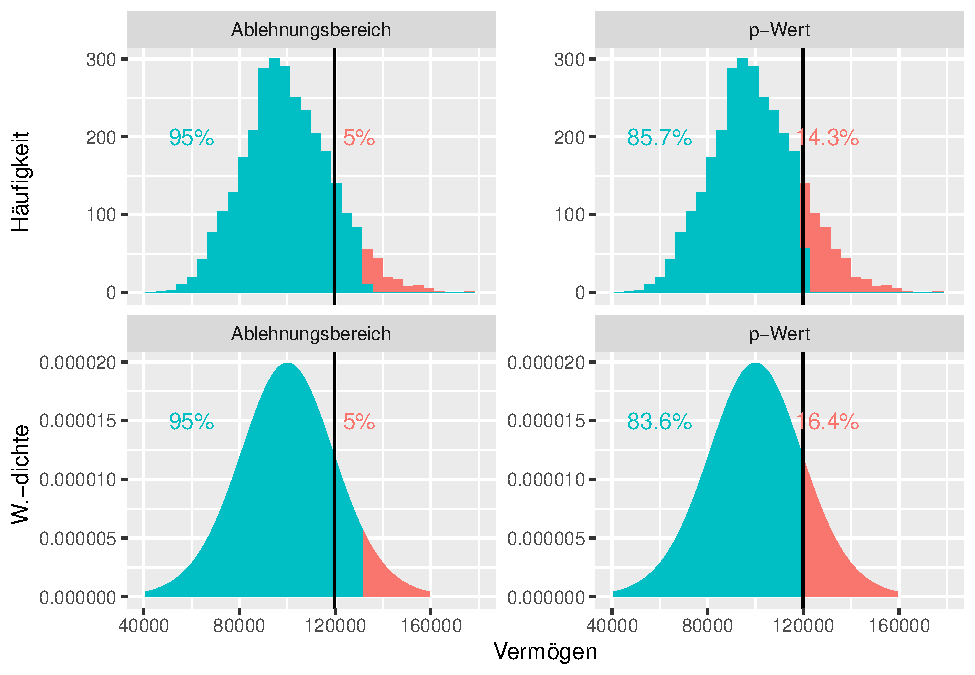
\includegraphics{aps_statistik1_files/figure-latex/exm-vermoegen-plots-sampling-theorie-1.pdf}
\caption{\label{fig:exm-vermoegen-plots-sampling-theorie}Oben: Histogramm der simulierten Verteilung; unten: theoretische t-Verteilung; links: Illustration p-Wert; rechts: Illustration Ablehnungsbereich. Die Linie entspricht dem beobachteten Stichprobenmittelwert.}
\end{figure}

\phantomsection\label{customdef-teststatistik}{Die Berechnung des für den Test relevanten Wertes, hier des \(t\)-Wertes wird \textbf{Teststatistik} (oder auch \emph{Prüfgrösse} oder nur \emph{Statistik}) genannt.} Eine Teststatistik hat normalerweise eine bekannte theoretische Verteilung, welcher die Teststatistik folgt, wenn die Nullhypothese wahr ist. \phantomsection\label{customdef-t-test}{Aufgrund der theoretischen \(t\)-Verteilung der Statistik wird dieser Test \textbf{\(t\)-Test} genannt.}

Das oben gefundene Resultat wird in der folgenden Form berichtet:

\begin{quote}
Das durchschnittliche Vermögen (\(M = 119853\) CHF, \(SD = 88528\), \(N = 20\)) ist in diesem Jahr nicht signifikant grösser als \(100'000\) CHF, \(t(19) = 1.003\), \(p = .164\).
\end{quote}

\begin{caution}

\begin{remark}

Folgende Begriffe und Zahlen werden dabei verwendet:

\begin{itemize}
\tightlist
\item
  Das \emph{durchschnittliche} Vermögen (fehlt durchschnittlich ist die Aussage falsch).
\item
  \(M\), \(SD\), \(N\) entsprechen dem arithmetischen Mittel, der geschätzten Standardabweichung und der Anzahl Beobachtungen in der Stichprobe. Die Einheit muss nicht wiederholt werden.
\item
  Signifikanz (siehe letzter Hinweis)
\item
  grösser als \(100'000\) CHF ist die Referenz zur Alternativhypothese
\item
  \(t(19)\) bedeutet, dass die Teststatistik \(t\)-verteilt ist mit \(19\) Freiheitsgraden.
\item
  \(1.003\) ist der Wert der Teststatistik berechnet mit Formel \eqref{eq:t-emp-onesample} aus der Stichprobe. Dieser Wert ist skaliert und muss im Kontext der standardisierten \(t\)-Verteilung wie in Abbildung \ref{fig:t-distribution} interpretiert werden.
\item
  \(p = .164\) entspricht dem \(p\)-Wert. Es wird normalerweise die führende \(0\) weggelassen (also nicht \(0.164)\), da es sich um eine Zahl handelt, welche nie kleiner als \(0\) oder grösser als \(1\) sein kann.
\end{itemize}

\end{remark}

\end{caution}

\begin{example}[Alexithymie]
\protect\hypertarget{exm:alexithymie}{}\label{exm:alexithymie}Mit Gefühlsblindheit oder \emph{Alexithymie} (griechisch: a = ohne, lexis= lesen, sprechen, thymie = Gefühle) werden Einschränkungen bei der Fähigkeit Emotionen wahrzunehmen, zu erkennen und zu beschreiben bezeichnet. Es gibt ein online \href{https://www.alexithymie.com/de/}{Messinstrument}, welches die Alexithymie auf einer Skala von \(37\) Punkten (kleine Gefühlsblindheit) bis \(185\) (grosse Gefühlsblindheit) misst. Die Skala wurde so gewählt, dass die durchschnittliche Alexithymie aller Menschen bei \(100\) liegt. Eine Psychologin interessiert sich nun dafür, ob junge Menschen unter \(25\) durchschnittlich andere Alexithymie-Werte aufweisen als die Gesamtbevölkerung. Um dies zu testen, befragt sie \(N = 391\) unter \(25\)-jährige mit besagtem Messinstrument. In dieser Gruppe wurde eine durchschnittliche Alexithymie von \(M = 96.7\) Punkten festgestellt.
\end{example}

Der erste Schritt ist auch hier die Null- und Alternativhypothesen aufzustellen. Die Psychologin stellt die Frage, ob sich die durchschnittliche Alexithymie in der Grundgesamtheit, in der Folge mit \(\mu\) bezeichnet, von \(100\) unterscheidet oder nicht. Es ist zu beobachten, dass sie keine Annahme über die Richtung der Abweichung trifft (eine höhere oder eine tiefere Alexithymie wären denkbar) und es sich deshalb um eine zweiseitige Hypothesenstellung handelt.

Die Nullhypothese beschreibt den bisherigen Informationsstand, also dass die durchschnittliche Alexithymie der Population bei \(100\) Punkten liegt, oder kurz

\begin{quote}
\(H_0:\mu = 100\) Punkte.
\end{quote}

Die Alternativhypothese besagt das Gegenteil davon, also hier, dass die durchschnittliche Alexithymie nicht mehr bei \(100\) Punkten liegt, oder kurz

\begin{quote}
\(H_1: \mu \neq 100\) Punkte.
\end{quote}

Um die Wahrscheinlichkeit des beobachteten arithmetischen Mittels der Stichprobe von \(M = 96.7\) Punkten zu ermitteln, gegeben, dass die Nullhypothese wahr ist, kann erneut auf eine Simulation zurückgegriffen werden. Bei diesem Gedankenexperiment wird angenommen, dass Nullhypothese wahr ist und dass das die Untersuchung \(4000\)-mal wiederholt wurde mit jeweils \(391\) Beobachtungen. Von jeder dieser Stichproben kann wiederum das arithmetische Mittel berechnet werden. Die Verteilung dieser arithmetischen Mittel ist in Abbildung \ref{fig:exm-alexithymie-plot} oben dargestellt.

\begin{verbatim}
## Warning: Removed 2 rows containing non-finite outside the scale range
## (`stat_bin()`).
\end{verbatim}

\begin{verbatim}
## Warning: Removed 8 rows containing missing values or values outside the scale range
## (`geom_bar()`).
\end{verbatim}

\begin{figure}
\centering
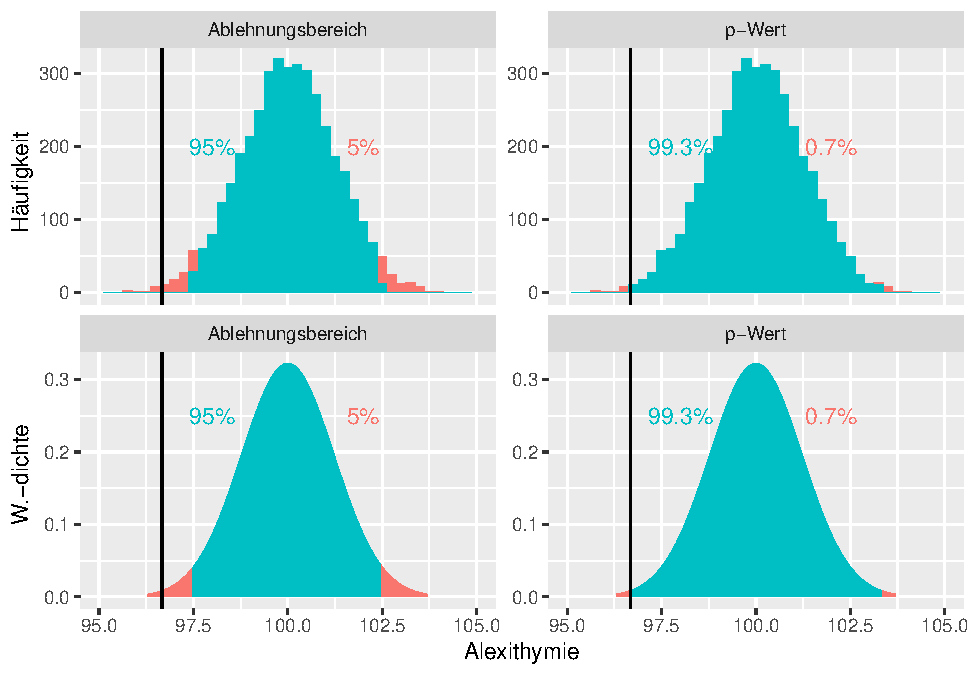
\includegraphics{aps_statistik1_files/figure-latex/exm-alexithymie-plot-1.pdf}
\caption{\label{fig:exm-alexithymie-plot}TODO:}
\end{figure}

Der \(p\)-Wert, also die Wahrscheinlichkeit, dass der beobachtete Wert oder ein noch extremerer Wert in Richtung der Alternativhypothese resultiert, wird hier aufgrund der zweiseitigen Hypothesenstellung auch zweiseitig ausgelegt. Extremer in Richtung der Alternativhypothese meint hier alle Werte, die weiter weg als der beobachtete Durchschnittswert \(96.7\) vom hypothetischen Erwartungswert \(\mu = 100\) sind. Konkret sind dies alle Werte, welche kleiner als \(96.7\), und alle Werte, welche grösser als \(103.3\) sind (roter Bereich in Abbildung \ref{fig:exm-alexithymie-plot} oben rechts). Der Anteil der Werte, welche diese Bedinung erfüllen liegt bei \(p = 0.7\%\). Es ist demnach recht unwahrscheinlich, dass die Nullhypothese stimmt und zufällig ein Stichprobendurchschnittswert von \(96.7\) Alexithymie-Punkten herauskommt.

Aufgrund der zweiseitigen Hypothesenstellung beinhaltet auch der Ablehnungsbereich sowohl die tiefsten \(2.5\%\) und höchsten \(2.5\%\), also insgesamt die \(5\%\) extremen Durchschnittswerte. Dies sind alle Werte tiefer als \(97.48\) und alle Werte höher als \(102.45\) (roter Bereich in Abbildung \ref{fig:exm-alexithymie-plot} oben links). Da das arithmetische Mittel der Stichprobe \(96.7\) im Ablehnungsbereich liegt, liegt hier ein signifikantes Resultat vor bei Signifikanzniveau \(5\%\).

Auch in diesem Fall kann die Verteilung der Stichprobenmittelwerte mit dem zentralen Grenzwertsatz angenähert werden. Es ergeben sich annähernd dieselben Resultate für den \(p\)-Wert (roter Bereich in Abbildung \ref{fig:exm-alexithymie-plot} unten rechts) und für den Ablehnungsbereich (roter Bereich in Abbildung \ref{fig:exm-alexithymie-plot} unten links).

Die Psychologin kann nun wie folgt berichten:

\begin{quote}
Die durchschnittliche Alexithymie (\(M = 96.7\) Punkte, \(SD = 24.4\), \(N = 391\)) unterscheidet sich bei den unter 25-jährigen signifikant vom Populationsdurchschnitt von \(100\) Punkte, \(t(390) = -2.698\), \(p = .007\).
\end{quote}

\section{Weicht der gefundene Durchschnitt stark vom hypothetischen Wert ab?}\label{weicht-der-gefundene-durchschnitt-stark-vom-hypothetischen-wert-ab}

In einem so berichteten Testresultat sind essenziell zwei Informationen enthalten: (1) was sind die getesteten Hypothesen und (2) wie wahrscheinlich es ist, dass das gefundene Resultat eine Folge der Zufallsstichprobenziehung ist. Was hier noch fehlt ist eine Angabe darüber wie gross die praktische Relevanz dieses Testresultates ist.

Um eine solche Relevanz zu messen wurde der Begriff der Effektstärke eingeführt. Eine Effektstärke ist eine Zahl ohne Einheit (Meter, Franken, \ldots), welche unabhängig von der Stichprobengrösse ist und nahe bei Null liegt, wenn die Nullhypothese nicht abgelehnt wurde.

Wird im Vermögensbeispiel \ref{exm:vermoegen} die Differenz zwischen geschätzem Erwartungswert und hypothetischem Erwartungswert
\[\bar{x} - \mu = 119853 \text{CHF} - 100000 \text{CHF}  = 19853\]
betrachtet, so fällt auf, dass dieser Wert bereits zwei der oben genannten Eigenschaften aufweist. Tatsächlich ist dieser Wert unabhängig von der Stichprobengrösse und er liegt nahe bei \(0\), wenn das Testresultat nicht signifikant war. Letzteres kann beobachtet werde indem in der Formel \eqref{eq:t-emp-onesample} verschiedene Differenzen eingesetzt werden und mit der Abbildung \ref{fig:t-distribution} verglichen werden.

Wenn jetzt ein anderer Sozialpsychologe die Auswertung wiederholen würde, aber statt in CHF in Rappen Rp rechnet, dann erhält er den Wert
\[\bar{x} - \mu = 11985300 \text{Rp} - 10000000 \text{Rp}  = 1985300.\]
Dass mit den gleichen Zahlen je nach Einheit eine andere Effektstärke gefunden wird ist unpraktisch für den Vergleich der Testresultate. Die Lösung in diesem Fall ist diese Differenz durch die geschätzte Standardabweichung zu rechnen. Dies ergibt

\begin{itemize}
\tightlist
\item
  in CHF: \(d = \frac{\bar{x} - \mu}{s} = \frac{119853 \text{CHF} - 100000 \text{CHF}}{88528\text{CHF}}  = 0.22\)
\item
  in Rp: \(d = \frac{\bar{x} - \mu}{s} = \frac{11985300 \text{Rp} - 10000000 \text{Rp}}{8852800\text{Rp}}  = 0.22 .\)
\end{itemize}

Mit dieser Formel werden für beide Einheiten derselbe Wert berechnet. Effektiv dient jetzt als Einheit die Standardabweichung: Eine grosse Differenz bei einer grossen Standardabweichung des Merkmals führt zur selben Effektstärke wie eine kleine Differenz bei kleiner Standardabweichung eines Merkmals. Da Menschen sich nicht gewohnt sind Zahlen als Standardabweichungen zu interpretieren hat \citep{cohen1988} ein folgende Richtwerte entwickelt:

\begin{itemize}
\tightlist
\item
  \(|d| \approx 0.3\): schwacher Effekt
\item
  \(|d| \approx 0.5\): mittlerer Effekt
\item
  \(|d| \approx 0.8\): starker Effekt
\end{itemize}

Cohen selbst hat davor gewarnt diese Werte als absolut darzustellen. Vielmehr sollte die Interpretation der Effektstärke vom Forschungsgebiet und dem Messinstrument abhängen. Um im Unterricht eine beurteilbare Praxis zu etablieren sollen folgende Regeln gelten:

\begin{itemize}
\tightlist
\item
  \(0 < |d| \leq 0.4\): schwacher Effekt
\item
  \(0.4 < |d| \leq 0.65\): mittlerer Effekt
\item
  \(0.65 < |d|\): starker Effekt
\end{itemize}

Das Berichten der Testresultate wird mit der Effektstärke ergänzt:

\begin{quote}
Das durchschnittliche Vermögen (\(M = 119853\) CHF, \(SD = 88528\), \(N = 20\)) ist in diesem Jahr nicht signifikant grösser als \(100'000\) CHF, \(t(19) = 1.003\), \(p = .164, d = 0.22\).
\end{quote}

\begin{quote}
Die durchschnittliche Alexithymie (\(M = 96.7\) Punkte, \(SD = 24.4\), \(N = 391\)) unterscheidet sich bei den unter 25-jährigen signifikant vom Populationsdurchschnitt von \(100\) Punkte, \(t(390) = -2.698\), \(p = .007, d = -0.14\).
\end{quote}

In beiden Fällen liegt ein schwacher Effekt vor. Der Effekt bei der Alexithymie ist schwächer als der Effekt bei der Vermögensstudie. Der \(p\)-Wert sagt aber aus, dass der Effekt beim Vermögen durch die Zufallsstichprobe zustande gekommen ist, während es bei der Alexithymie unwahrscheinlich ist, dass der Effekt durch die Zufallsstichprobe zustande gekommen ist.

\section{Übungen}\label{uxfcbungen-2}

\begin{exercise}
\protect\hypertarget{exr:vermoegen}{}\label{exr:vermoegen}\leavevmode

Reproduziere das Beispiel Vermögen \ref{exm:vermoegen} mit \texttt{Jamovi} indem folgende Teilschritte durchgeführt werden:

\begin{itemize}
\tightlist
\item
  Datensatz \texttt{05-exm-vermoegen.sav} in \texttt{Jamovi} einladen.
\item
  Wähle \texttt{Analysen\ \textgreater{}\ t-Tests\ \textgreater{}\ t-Test\ mit\ einer\ Stichprobe}.
\item
  Definiere die Hypothese wie im Beispiel und wähle die Testoptionen so, dass du alle Zahlen des Testberichts wiederfindest.
\end{itemize}

\end{exercise}

\begin{solution}
\leavevmode

\begin{figure}
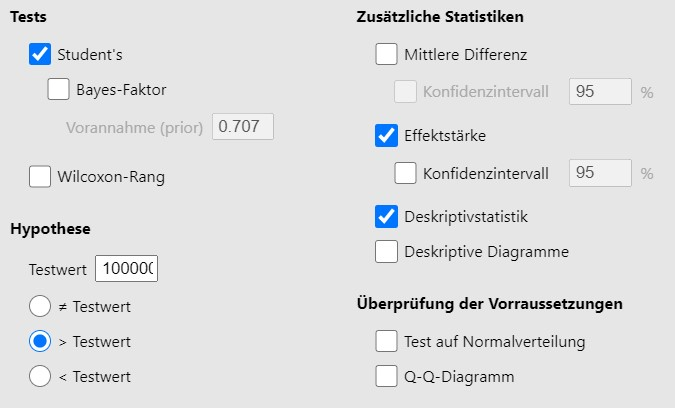
\includegraphics[width=1\linewidth]{figures/05-exr-vermoegen-jmv-input} \caption{Jamovi Eingabe.}\label{fig:sol-vermoegen-input}
\end{figure}

\begin{figure}
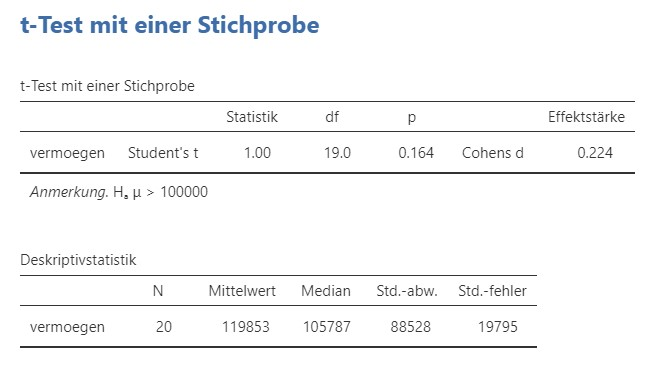
\includegraphics[width=1\linewidth]{figures/05-exr-vermoegen-jmv-output} \caption{Deskriptive Statistiken.}\label{fig:sol-vermoegen-output}
\end{figure}

\end{solution}

\begin{exercise}
\protect\hypertarget{exr:alexithymie}{}\label{exr:alexithymie}\leavevmode

Reproduziere das Beispiel Alexithymie \ref{exm:alexithymie} mit \texttt{Jamovi} indem folgende Teilschritte durchgeführt werden:

\begin{itemize}
\tightlist
\item
  Datensatz \texttt{05-exm-alexithymie.sav} in \texttt{Jamovi} einladen.
\item
  Wähle \texttt{Analysen\ \textgreater{}\ t-Tests\ \textgreater{}\ t-Test\ mit\ einer\ Stichprobe}.
\item
  Definiere die Hypothese wie im Beispiel und wähle die Testoptionen so, dass du alle Zahlen des Testberichts wiederfindest.
\end{itemize}

\end{exercise}

\begin{solution}
\leavevmode

\begin{figure}
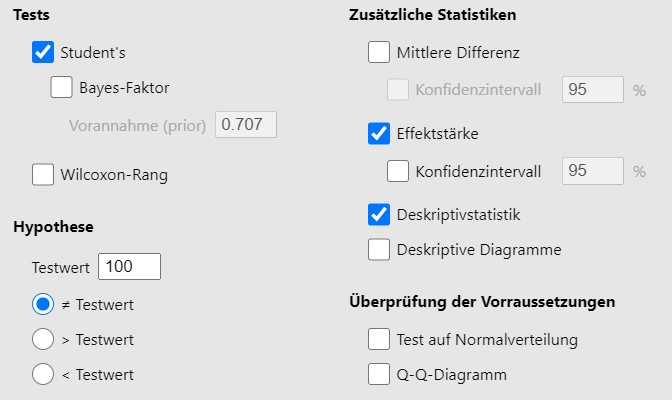
\includegraphics[width=1\linewidth]{figures/05-exr-alexithymie-jmv-input} \caption{Jamovi Eingabe.}\label{fig:sol-alexithymie-input}
\end{figure}

\begin{figure}
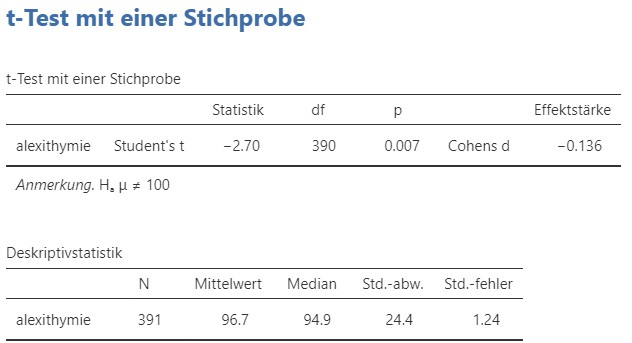
\includegraphics[width=1\linewidth]{figures/05-exr-alexithymie-jmv-output} \caption{Deskriptive Statistiken.}\label{fig:sol-alexithymie-output}
\end{figure}

\end{solution}

\part{Gruppenvergleich einer intervallskalierten Variable}\label{part-gruppenvergleich-einer-intervallskalierten-variable}

\chapter{Gruppenvergleich einer intervallskalierten Variable}\label{gruppenvergleich-einer-intervallskalierten-variable}

\section{Zwei Gruppen vergleichen}\label{zwei-gruppen-vergleichen}

\section{Was ist das Problem der Stichprobenziehung?}\label{was-ist-das-problem-der-stichprobenziehung}

\section{Wie kann man Aussagen über die Grundgesamtheit machen?}\label{wie-kann-man-aussagen-uxfcber-die-grundgesamtheit-machen}

\section{Übungen}\label{uxfcbungen-3}

\chapter{Welch-Test}\label{welch-test}

\section{Zwei Gruppen vergleichen}\label{zwei-gruppen-vergleichen-1}

\section{Sind die Durchschnitte der beiden Gruppen in der Grundgesamtheit gleich?}\label{sind-die-durchschnitte-der-beiden-gruppen-in-der-grundgesamtheit-gleich}

\section{Wie stark unterscheiden sich die Durchschnitte?}\label{wie-stark-unterscheiden-sich-die-durchschnitte}

\section{Übungen}\label{uxfcbungen-4}

\chapter*{Begriffsverzeichnis}\label{begriffsverzeichnis}
\addcontentsline{toc}{chapter}{Begriffsverzeichnis}

\begin{itemize}
\tightlist
\item
  \hyperref[customdef-alternativhypothese]{Alternativhypothese}
\item
  \hyperref[customdef-erwartungswert]{Erwartungswert}
\item
  \hyperref[customdef-freiheitsgrade]{Freiheitsgrade}
\item
  \hyperref[customdef-grundgesamtheit]{Grundgesamtheit}
\item
  \hyperref[customdef-hypothese]{Hypothese}
\item
  \hyperref[customdef-iqr]{Interquartilabstand}
\item
  \hyperref[customdef-interval]{Intervalles}
\item
  \hyperref[customdef-confidence-interval]{Konfidenzintervall}
\item
  \hyperref[customdef-median]{Median}
\item
  \hyperref[customdef-modus]{Modus}
\item
  \hyperref[customdef-normalverteilung]{Normalverteilung}
\item
  \hyperref[customdef-nullhypothese]{Nullhypothese}
\item
  \hyperref[customdef-perzentil]{Perzentil}
\item
  \hyperref[customdef-population]{Population}
\item
  \hyperref[customdef-spannweite]{Spannweite}
\item
  \hyperref[customdef-std]{Standardabweichung}
\item
  \hyperref[customdef-stichprobe]{Stichprobe}
\item
  \hyperref[customdef-stichprobenziehung]{Stichprobenziehung}
\item
  \hyperref[customdef-student-verteilung]{Student-\(t\)-Verteilung}
\item
  \hyperref[customdef-zentraler-grenzwertsatz]{Zentraler Grenzwertsatz}
\item
  \hyperref[customdef-zufallsstichprobe]{Zufallsstichprobe}
\item
  \hyperref[customdef-arithmetisches-mittel]{arithmetische Mittel}
\item
  \hyperref[customdef-intervallskaliert]{intervallskaliert}
\item
  \hyperref[customdef-zweiseitige-hypothese]{zweiseitige Hypothese}
\end{itemize}

  \bibliography{book.bib,packages.bib}

\end{document}
